%\documentclass[11pt,a4paper,uplatex,dvipdfmx]{ujarticle} 		% for uplatex
\documentclass[11pt,a4j,dvipdfmx]{jarticle} 					% for platex
%=======================================
% form00_header.tex
%	General header for kakenhiLaTeX,  Moved over from form00_2010_header.tex.
%	2009-09-06 Taku Yamanaka (Osaka Univ.)
%==== General Version History ======================================
% 2006-05-30 Taku Yamanaka (Physics Dept., Osaka Univ.)
% 2006-06-02 V1.0
% 2006-06-14 V1.1 Use automatic calculation for cost tables.
% 2006-06-18 V1.2 Split user's contents and the format.
% 2006-06-20 V1.3 Reorganized user and format files
% 2006-06-25 V1.4 Readjusted all the table column widths with p{...}.
%				With \KLTabR and \KLTabRNum, now the items can be right-justified
%				in the cell defined by p{...}.
% 2006-06-26 V1.5 Use \newlength and \setlength, instead of \newcommand, to define positions.
% 2006-08-19 V1.6 Remade it for 2007 JFY version.
% 2006-09-05 V1.7 Added font declarations suggested by Hoshino@Meisei Univ.
% 2006-09-06 V1.8 Introduced usePDFform flag to switch the form file format.
% 2006-09-09 V1.9 Changed p.7, to allow different heights between years. (Thanks to Ytow.)
% 2006-09-11 V2.0 Added an option to show budget summary.
% 2006-09-13 V2.1 Added an option to show the group.
% 2006-09-14 V2.1.1 Cleaned up Kenkyush Chosho.
% 2006-09-21 V2.2 Generated under a new automatic development system.

% 2007-03-24 V3.0 Switched to a method using "picture" environment.

% 2007-08-14 V3.1 Switched to kakenhi3.sty.
% 2007-09-17 V3.2 Added \KLMaxYearCount
% 2008-03-08 V3.3 Remade it for 2009 JFY version\
% 2008-09-08 V3.4 Added \KLXf ... \KLXh.
% 2011-10-20 V5.0 Use kakenhi5.sty, to utilize array package in tabular environment.
% 2012-08-14 v5.1 Moved preamble and kakenhi5 into the current directory, instead of the parent directory.
% 2012-11-10 v6.0 Switched to kakenhi6.sty.
% 2015-08-26 v6.1 Added KLFirstPageIsLongPage flag.
% 2017-05-27 v7.0 Simplified for the new format.
% 2022-10-27 v7.1 Removed [dvipdfmx] from \usepackage{graphicx}.
%=======================================
% Dummy section and subsection commands.
% With these, some editors (such as TeXShop, etc.) can jump to the (sub)sections.
\newcommand{\dummy}{dummy}% 
\renewcommand{\section}[1]{\renewcommand{\dummy}{#1}}

\usepackage{calc}
\usepackage{geometry}                % See geometry.pdf to learn the layout options. There are lots.
\usepackage{graphicx}
\usepackage{color}
\usepackage{ifthen}
\usepackage{udline}
\usepackage{array}
\usepackage{longtable}
\usepackage{fancyhdr}
 % pieces
%==================================================
% kakenhi7.sty
%==================================================
% v1
% Minimum amount of macros for writing Kakenhi forms.
%
% 2005-10-24 Taku Yamanaka, Physics Dept. Osaka Univ.
%		taku@hep.sci.osaka-u.ac.jp
% 		Macros such as XYBC, etc. were imported from Kakenhi Macro at
% 		http://www.yukawa.kyoto-u.ac.jp/contents/researcher/kakenhi.html .
% 2006-06-04 Taku
%		Added macros to draw boxes if \DrawBox is in the source.
%		This is useful when designing the LaTeX forms.
% 2006-06-14 Taku
%		Added LaTeX macros to add costs 
%		(\KLResetGrandSum, \KLCostItem, \KLSum, \KLGrandSum).
%		Added a macro \Number to supply commas every 3 digits (imported from kkh.mac).
% 2006-06-25 Taku
%		Added \KLTabC, \KLTabR, \KLTabRNum to specify alignments in tables.
%		Please note that \phantom{...} is required for the column, 
%		or otherwise somehow p{...mm} is ignored.
% 2006-08-13 Taku
%		Added \KLItemNumUnitCost . This requires calc.sty.
% 2006-09-06 Taku
%		Added KLGrandTotalValue to add ALL the costs.
%		Also added \KLPrintGrandTotal to print the total on the console.
% 2006-09-09 Taku
%		Added macros to handle "efforts".
% 2006-09-10 Taku
%		Added \KLnewcounter to make series of counters.
%		Modified \KLResetGrandSum and \KLSum to add the sum for 
%		each category and year.
% 2006-09-11 Taku
%		Added \NumC to display LaTeX counter with commas.
% 2006-09-12 Taku
%		Added simple macros to make group table.
% 2006-09-23 Taku
%		Added the 'Fair License' notification.
% 2006-10-22 Taku
%		Initialize KLNumPeople to -1, so that the first header row will not be included in the count.
%====================================================
% v2
% 2007-03-24 Taku
%		Instead of using Kakenhi Macros to position items, 
%		switched to a new method using
%		"picture" environment.  The origin of the coordinate is set to 
%		the lower left corner of the paper.  The positions are given in "points", 
%		as can be read by gv. These methods were suggested by 
%		Tsutomu Sakurai at Saitama Univ..
% 2007-03-30 Taku
%		The sum of each category and year is made using 
%		macros \KLItemCost, etc., instead of \KLSum.  This is a step toward
%		automatically aligning category sums in the same year, in some forms.
% 2007-04-02 Taku
%		Added \KLBudgetMiniTabular, \KLMiniSum, etc. to handle
%		budget tables with multiple category columns.
% 2007-05-04 Taku
%		Added \multicolumnDottedLine .
%==================================================
% v3 
% 2007-08-14 Taku
%		Simplified page handling, by introducing \KLBeginSinglePage,
%		\KLPageRange, etc..
% 2007-09-01 Taku
%		Added a new command, \KLItemNumUnitCostLocation , 
%		and \KLAddCost to clean things up.
% 2007-09-06 Taku
%		Set \KLEven/OddLeft/RightEdge parameters in \KLWaterMark.
%		Without it, if \KLLeftEdge or \KLRightEdge is used inside watermark,
%		it generated a very obscure error message, which was hard to track down.
% 2007-09-09 Taku
%		Removed clearring \thiswatermark in \KLClearWaterMarks.
% 2007-09-12 Taku
%		Added \KLPriorityItemNumUnitCostTwo for Tokusui.
% 2007-09-14 Taku
%		Added \KLItemNumUnitCostTwo for tokutei_koubo.
% 2007-09-17 Taku
%		In \KLAddCost, costs are added only if it is within the defined year range.
% 2008-09-02 Taku
%		  Added \KLMonthPriorityItemNumUnitCostTwo for tokutei_keizoku.
% 2008-09-07 Taku
%		   Use \KLJFY to print year in budget tables.
% 2008-10-21 Taku
%			Added KLItemNumUnitCostInParen for shorei.
% 2009-09-03 Taku
%			Added \dottedLine .
%==================================================
% v4
% 2009-09-06 Taku
%			Added macros for partial typesetting.
% 2009-09-12 Taku
%			Added macros for showing coordinates and edges.
% 2009-09-13 Taku
%			Added macros to show boxes and minipage frames and their corner coordinates.
% 2010-03-04 Taku
%			Moved macros for calculating lengths and positions from form07_header.tex to here.
% 2010-04-11 Taku
%			Added \KLItemCostOne for jisedai, and necessary flags to print budget sums before 
%			the detailed budget table.
%==================================================
% v5
% 2011-10-20 Taku
%			By using array package within tabular environment, the following macros were simplified:
%			\KLTabC, \KLTabR, \KLBudgetMiniTabular, 
%			New Macros:
%			\KLCC, \KLCR
% 2011-10-24 Taku
%			Removed using \KLTabR from most of the budget tables.
% 2011-10-26 Taku
%			Added KLMyBudget.
%			Modified KLYearItemNumUnitCostTwo to just put the JFY if the second item is blank.  (For Kiban S)
% 2012-03-10 Taku
%			Changed the tabcolsep for \KLMyBudget to 0pt.
% 2012-08-14 Taku
%			Moved xxx_forms_pdf and _eps directories to under mother.
% 2012-09-09	Taku
%			Added \KLbibitem(B) and \KLcite(B).
% 2012-09-16	Taku
%			Added \KLOtherApplication, \KLOtherApplicationReasons, and \KLOtherFundReasons
%			for tokusui (and maybe for others in the future).
%==================================================
% v6
% 2012-11-10	Taku
% 			Modified \KLOtherApplicationReasons and \KLOtherFundReasons to make the tables compact.
%			These were in hook3.tex for the 2013 version.
%			Added \KLOtherApplicationDiff for many shumokus.
%			Removed \KLbibitemB and \KLciteB.
%			Changed \KLbibitem to use a dedicated column for numbering.
% 2012-11-11	Taku
%			Added \KLItemSetCostLocationInfo and \KLItemCostInfo.
% 2013-09-19	Taku
%			Added \KLOtherPD and \KLOtherPDShort to enter JSPS PD for other funds.
% 2013-10-02	Taku
%			Changed \KLbibItem, not to use a dedicated column for numbering, 
%			because otherwise the label defined in \label{...} cannot be used in @currentlabel.
% 2014-09-22	Taku
%			Added \KLCL for filling narrow tabular cells in English.  
%			(Suggested by Frank Bennett.)
% 2014-11-08	Taku
%			Added an instruction in \KLCheckPageLimit.
% 2015-08-23	Taku
%			Added NumCk to show numbers divided by 1000 (truncated).
% 2015-08-24	Taku
%			Introduced \KLLongPage and \KLSimpleLongPage to offer floating environment in 
%			single-page-frames.
%=====================================================
% v7
%	Frames are gone!  Simplify kakenhiLaTeX to benefit from 
%	the new style.
% 2017-05-03	Taku
%			Added \KLAnotherFund .
% 2017-05-27	Taku
%			Made \KLBeginSubject and \KLEndSubject to handle new 
%			mother file style.
% 2017-08-17 Taku
%	Added \KLItemCostNoYear and \KLEndBudgetNoYear for kokusai_kyoudou.
% 2017-08-19	Taku
%			Updated \KLBeginSubject and \KLEndSubject to handle 
%			various headers.
% 2017-08-20	Taku
%			\KLBeginSubject calls \KLFirstPageStyle and \KLDefaultPageStyle
%			which should be defined for each shumoku (or JSPS/MEXT).
%			This is to pass the subject name etc. to the header.
% 2017-08-27	Taku
%			Set section number in \KLBeginSubject.
% 2017-08-29	Taku
%			Moved over KLShumokuFirstPageStyle and KLShumokuDefaultPageStyle.
%			Added jsps-abs-p1-header, jps-abs-subject-header, and 
%			jsps-abs-default-header as arguments to \KLShumoku***Header.
% 2017-09-02	Taku
%			Added \KLBeginSubjectWithHeaderCommands for more flexible header style.
% 2017-09-03	Taku
%			Added \vspace*{-4mm} after \includegraphics in \KLBeginSubject*.
% 2017-09-05	Taku
%			Removed now-the-old commands.
% 2020-01-02	Taku
%			Added more numbers to \KLJint for gakuhen_a.
% 2020-01-15	Taku
%			Changed the horizontal position (none --> -3mm) 
%			and the width of the top boxes for headers (\linewidth --> 1.02\linewidth)
%			to reproduce the original boxes.  
%			This became necessary because the margins were set correctly in form02_header.tex.
% 2021-01-29	Taku
%			Set section counter and reset subsection counter only if the section # is given for
%			\KLBeginSubject and \KLBeginSubjectWithHeaderCommands .
% 2022-01-26	Taku
%			Changed the scale for the top boxes from 1.03 to 1.01, 
%			and \hspace from -3mm to -2mm.  (DC)
% 2022-02-23	Taku
%			Introduced \KLBoxOffset and \KLBoxScale for flexibility.
% 2022-03-20	Taku
%			Added '%' after \hspace{ } before incldegraphics.
% 2022-08-03	Taku
%			Use width=\KLBoxWidth, instead of \KLBoxScale*\linewidth which depents on
%			\linewidth.  (I should have noticed it earlier.)
% 2023-03-09	Taku
%			Added \vspace*{\KLBoxVOffset} to \KLBeginSubject.
% 2023-07-10	Taku
%			Added \includegraphics_full_width to place full-width 
%			instruction box images.
%			This is used also for \KLBeginSubject and 
%			\KLBeginSubjectWithHeaderCommands.  
%			\KLBoxOffset and \KLBoxWidth are not needed anymore.
%			Why didn't I think of it (-1in-\oddsidemargin) before??
% 2023-07-18	Taku
%			Old LaTeX cannot handle \hspace{-1in-\oddsidemargin}.
%			Changed to calculate the length by \setlength, and then use the result in \hspace.
%=====================================================

%=====================================================
% Macro to supply commas every 3 digits (up to 9 digits)
%	Imported from kkh.mac for Kakenhi Macro.
%=====================================================
%
\newif\ifNumWithCommas \NumWithCommastrue
\def\NumWithCommas{\NumWithCommastrue}
\def\NumWithoutCommas{\NumWithCommasfalse}
\newcount\Numa
\newcount\Numb
\def\Numempty{}%output blank if "-0" is given
\def\Number#1{\edef\Numpar{#1}\ifx\Numempty\Numpar\else%
\ifNumWithCommas\Numa=#1\relax
\ifnum\Numa>999999\divide\Numa by 1000000
\number\Numa,%
\multiply\Numa by -1000000\advance\Numa by #1\relax
\Numb=\Numa\divide\Numa by 1000
\ifnum\Numa<100 \ifnum\Numa<10 0\fi0\fi\number\Numa,%
\multiply\Numa by -1000\advance\Numa by \Numb
\ifnum\Numa<100 \ifnum\Numa<10 0\fi0\fi\number\Numa%
\else\ifnum\Numa>999\divide\Numa by 1000
\number\Numa,%
\multiply\Numa by -1000\advance\Numa by #1\relax
\ifnum\Numa<100 \ifnum\Numa<10 0\fi0\fi\number\Numa%
\else\number\Numa\fi\fi\else\number#1\fi\fi}

%======================================================
% Macro to display LaTeX counter with commas every 3 digits.
%======================================================
\newcommand{\NumC}[1]{\Number{\value{#1}}}

\newcounter{kyen}
\newcommand{\NumCk}[1]{%
	\setcounter{kyen}{\arabic{#1}/1000}
	\Number{\value{kyen}}
}

%======================================================
% Macros to align (right-justify, center) elements within a tabular cell
% whose width is defined by p{...}.
% 2006-06-25 Taku
% 	These are necessary, because the cell width should be given explicitly
% 	by p{...mm} to match the given table in a tabular environment.  
% 	One could allocate a width with \phantom{...},
% 	but it is a little tricky, since it depends on the font size.
%======================================================

%---------------------------------------------------------------------
% Center text within a tabular cell allocated by p{...}
%\newcommand{\KLTabC}[1]{\multicolumn{1}{c}{#1}}
\newcommand{\KLTabC}[1]{\centering\arraybackslash#1}
% This new method does not require a dummy table row to put them in correct columns.
%
% This should be used in tabular definition, as:
%	\begin{tabular}[t]{>{\KLCC}p{30pt}p{50pt}}
\newcommand{\KLCC}{\centering\arraybackslash}

%---------------------------------------------------------------------
% Right justify text within a tabular cell allocated  by p{...}
%\newcommand{\KLTabR}[1]{\multicolumn{1}{r@{\ }}{#1}}
\newcommand{\KLTabR}[1]{\raggedleft\arraybackslash#1}

% This should be used in tabular definition, as:
%	\begin{tabular}[t]{>{\KLCR}p{30pt}p{50pt}}
\newcommand{\KLCR}{\raggedleft\arraybackslash}%

%---------------------------------------------------------------------
% Right justify number (with comma every 3 digits) 
% within a tabular cell allocated by p{...}
\newcommand{\KLTabRNum}[1]{\KLTabR{\Number{#1}}}

%---------------------------------------------------------------------
% Left justify text within a tabular cell allocated by p{...}
% This should be used in tabular definition, as:
%	\begin{tabular}[t]{>{\KLCL}p{30pt}p{50pt}}
\newcommand{\KLCL}{\raggedright\arraybackslash}%

%=================================================
%  counter tools
%=================================================
\newcounter{KLtmp}

%------------------------------------------------------------------------------
% Makes a set of counters, with prefix #1, followed by 
% suffix ranging from 0 to #2 - 1.
% For example, \KLnewcounter{mine}{3} makes counters
% mine0, mine1, and mine2 .
%-------------------------------------------------------------------------------
\newcommand{\KLnewcounter}[2]{
	\setcounter{KLtmp}{0}
	
	\whiledo{\value{KLtmp} < #2}{
		\newcounter{#1\arabic{KLtmp}}
		\stepcounter{KLtmp}
	}
}

%------------------------------------------------------------------------------
% Dumps the contents of the counters.
%------------------------------------------------------------------------------
\newcommand{\KLdumpcounter}[2]{
	\setcounter{KLtmp}{0}
	
	\whiledo{\value{KLtmp} < #2}{
		#1\arabic{KLtmp} : \arabic{#1\arabic{KLtmp}}\\
		\stepcounter{KLtmp}
	}
}

%=======================================================
% LaTeX macros to add costs.
%	2006-06-14 Taku Yamanaka
%=======================================================
\newcounter{KLCost}				% to calculate cost = #units x unit cost
\newcounter{KLGrandTotalValue}		% for the grand total of all the categories in all years
\setcounter{KLGrandTotalValue}{0}

\newcommand{\KLCostCategory}{KLequipments}
\newcounter{KLYearCount}
\newcounter{KLPrintYear}

% Make counters for annual sums for each category-----------------------
\newcommand{\KLMaxYear}{8}
\KLnewcounter{KLequipments}{\KLMaxYear}
\KLnewcounter{KLexpendables}{\KLMaxYear}
\KLnewcounter{KLdomestic}{\KLMaxYear}
\KLnewcounter{KLforeign}{\KLMaxYear}
\KLnewcounter{KLtravel}{\KLMaxYear}
\KLnewcounter{KLgratitude}{\KLMaxYear}
\KLnewcounter{KLmisc}{\KLMaxYear}
\KLnewcounter{KLAnnualSum}{\KLMaxYear}

%------------------------------------------------
% Add up the given cost to category-year sum, category sum, year-sum, and total.
% 2007-09-01 Taku
% 2007-09-17 Taku: Add costs only if it is within the defined year range.
%------------------------------------------------
\newcommand{\KLAddCost}[1]{%
	\ifthenelse{\value{KLYearCount} > \value{KLMaxYearCount}}{%
		%pass
	}{%
		\addtocounter{\KLCostCategory0}{#1}%
		\addtocounter{\KLCostCategory\arabic{KLYearCount}}{#1}%
		\addtocounter{KLAnnualSum\arabic{KLYearCount}}{#1}%
		\addtocounter{KLAnnualSum0}{#1}%
		\ifthenelse{\equal{\KLCostCategory}{KLdomestic}}{%
			\addtocounter{KLtravel0}{#1}%
			\addtocounter{KLtravel\arabic{KLYearCount}}{#1}%
		}{}%
		\ifthenelse{\equal{\KLCostCategory}{KLforeign}}{%
			\addtocounter{KLtravel0}{#1}%
			\addtocounter{KLtravel\arabic{KLYearCount}}{#1}%
		}{}%
	}%
}


\newcommand{\KLClearWaterMarks}{%
	%--empty watermarks
	\watermark{}
%	\thiswatermark{}
	\rightwatermark{}
	\leftwatermark{}
}

\newcommand{\KLInput}[1]{%	The macros defined inside the file are only valid within the file.
	\begingroup
	\input{#1}
	\endgroup
}

%================================
% For 2017 new style without frames
%================================
\newcommand{\KLShumokuFirstPageStyle}[5]{%
%	Defines the header for the first page.
%	Called from \KLBeginSubject.
%--------------------------------
%	#1: page style name
%	#2: 様式
%	#3: 研究種目名
%	#4: 項目名
%	#5: sectionNo
%--------------------------------
	\ifthenelse{\equal{#1}{jsps-p1-header}}{%
		\JSPSVeryFirstPageStyle{#1}{#2}{#3}{#4}{#5}
	}{%
		\ifthenelse{\equal{#1}{jsps-abs-p1-header}}{%
			\JSPSVeryFirstPageStyle{#1}{#2}{#3 概要}{#4}{#5}
		}{%
            		\ifthenelse{\equal{#1}{jsps-subject-header}}{%
            			\JSPSFirstSubjectPageStyle{#1}{#2}{#3}{#4}{#5}
            		}{%
				\ifthenelse{\equal{#1}{jsps-abs-subject-header}}{%
            				\JSPSFirstSubjectPageStyle{#1}{#2}{#3 概要}{#4}{#5}
				}{%
                    			\thispagestyle{#1}
				}
            		}
		}
	}
}

\newcommand{\KLShumokuDefaultPageStyle}[5]{%
%	Defines the default header.
%	Called from \KLBeginSubject.
%--------------------------------
%	#1: page style name
%	#2: 様式
%	#3: 研究種目名
%	#4: 項目名
%	#5: sectionNo
%--------------------------------
	\ifthenelse{\equal{#1}{jsps-default-header}}{%
		\JSPSDefaultPageStyle{#1}{#2}{#3}{#4}{#5}
	}{%
		\ifthenelse{\equal{#1}{jsps-abs-default-header}}{%
			\JSPSDefaultPageStyle{#1}{#2}{#3 概要}{#4}{#5}
		}{%
            		\pagestyle{#1}
		}
	}
}

\newcommand{\KLSubjectName}{}
\newcommand{\KLSubjectMaxPages}{}
\newcommand{\KLSubjectEndPage}{}
\newcounter{KLSubjectEndPage}
\setcounter{KLSubjectEndPage}{0}

\newcommand{\KLSubjectCheckNPages}{%
%	\arabic{page}, \arabic{KLSubjectEndPage}\\
	\ifthenelse{\value{page}>\value{KLSubjectEndPage}}{
		{\LARGE「\KLSubjectName」は \KLSubjectMaxPages\ ページ以内で書いてください。}
		\clearpage
	}{%
	}
}

\newcommand{\KLSubjectAdvancePages}{%
	\renewcommand{\KLSubjectEndPage}{\value{KLSubjectEndPage}}
	\ifthenelse{\value{page}<\KLSubjectEndPage}{%
		\phantom{x}\clearpage
	}{}
	% Advance page if necessary
	\ifthenelse{\value{page}<\KLSubjectEndPage}{%
		\phantom{x}\clearpage
	}{}
	% Advance page if necessary
	\ifthenelse{\value{page}<\KLSubjectEndPage}{%
		\phantom{x}\clearpage
	}{}
	% Advance page if necessary
	\ifthenelse{\value{page}<\KLSubjectEndPage}{%
		\phantom{x}\clearpage
	}{}
	% Advance page if necessary
	\ifthenelse{\value{page}<\KLSubjectEndPage}{%
		\phantom{x}\clearpage
	}{}
}	

\newcommand{\KLJInt}[1]{%
% Returns full-width numerical character.
	\ifthenelse{\equal{#1}{1}}{1}{%
	\ifthenelse{\equal{#1}{2}}{2}{%
	\ifthenelse{\equal{#1}{3}}{3}{%
	\ifthenelse{\equal{#1}{4}}{4}{%
	\ifthenelse{\equal{#1}{5}}{5}{%
	\ifthenelse{\equal{#1}{6}}{6}{%
	\ifthenelse{\equal{#1}{7}}{7}{%
	\ifthenelse{\equal{#1}{8}}{8}{%
	\ifthenelse{\equal{#1}{9}}{9}{%
	\ifthenelse{\equal{#1}{10}}{10}{%
	\ifthenelse{\equal{#1}{11}}{11}{%
	\ifthenelse{\equal{#1}{12}}{12}{%
	\ifthenelse{\equal{#1}{13}}{13}{%
	\ifthenelse{\equal{#1}{14}}{14}{%
	\ifthenelse{\equal{#1}{15}}{15}{%
	\ifthenelse{\equal{#1}{16}}{16}{%
	\ifthenelse{\equal{#1}{17}}{17}{%
	#1}}}}}}}}}}}}}}}}}%
}

\newlength{\KLFWHOffset}

\newcommand{\includegraphicsFullWidth}[1]{%
	\noindent%
%	\hspace{-1in-\oddsidemargin}%	New LaTeX (2020) can handle this, but old ones (2018) cannot.
	\setlength{\KLFWHOffset}{-1in-\oddsidemargin}%
	\hspace{\KLFWHOffset}%		For old LaTeX
	\includegraphics[width=\paperwidth]{#1}%
}

\newcommand{\KLBeginSubject}[8]{%
%----------------------------------------------------
%	#1: subjectNo
%	#2: sectionNo
%	#3: sectionJ
%	#4: maxPages
%	#5: pageLengthStyle ('V' for variable, 'F' for fixed)
%	#6: pageCounter (set page counter to this value if the argument exists.
%	#7: subjectFirstPageHeader (header for the first page)
%	#8: defaultPageHeader
%----------------------------------------------------
	\ifthenelse{\equal{#2}{}}{%
	}{%
	    	\setcounter{section}{#2}
	    	\setcounter{subsection}{0}
	}
	\setcounter{subsubsection}{0}
	\renewcommand{\KLSubjectName}{#3}
	\renewcommand{\KLSubjectMaxPages}{#4}
	
	\ifthenelse{\equal{#6}{}}{%
	}{%
		\setcounter{page}{#6}
	}
	
	\setcounter{KLSubjectEndPage}{\value{page}}
	\addtocounter{KLSubjectEndPage}{#4}
	
	\ifthenelse{\equal{#7}{}}{%
		% pass
	}{%
		\KLShumokuFirstPageStyle{#7}{\様式}{\研究種目header}{#3}{#2}
	}
	
	\ifthenelse{\equal{#8}{}}{%
		% pass
	}{%
		\KLShumokuDefaultPageStyle{#8}{\様式}{\研究種目header}{#3}{#2}
	}
	
	\vspace*{\KLBoxVOffset}%
%	\noindent
%	\hspace{\KLBoxOffset}%
%	\includegraphics[width=\KLBoxScale\linewidth]{subject_headers/\KLYoshiki_#1.pdf}\\
	\includegraphicsFullWidth{subject_headers/\KLYoshiki_#1.pdf}
	\vspace*{-4mm}
}

\newcommand{\KLNullHeader}[5]{}
% Dummy command for No header.
% This was introduced to avoid error caused in statement \ifthenelse{\equal{#8}{}} .

\newcommand{\KLBeginSubjectWithHeaderCommands}[8]{%
%----------------------------------------------------
%	#1: subjectNo
%	#2: sectionNo
%	#3: sectionJ
%	#4: maxPages
%	#5: pageLengthStyle ('V' for variable, 'F' for fixed)
%	#6: pageCounter (set page counter to this value if the argument exists.
%	#7: LaTeX command for subjectFirstPageHeader (header for the first page)
%	#8: LaTeX command for defaultPageHeader
%----------------------------------------------------
	\ifthenelse{\equal{#2}{}}{%
	}{%
		\setcounter{section}{#2}
		\setcounter{subsection}{0}
	}
	\setcounter{subsubsection}{0}
	\renewcommand{\KLSubjectName}{#3}
	\renewcommand{\KLSubjectMaxPages}{#4}
	
	\ifthenelse{\equal{#6}{}}{%
	}{%
		\setcounter{page}{#6}
	}

	\setcounter{KLSubjectEndPage}{\value{page}}
	\addtocounter{KLSubjectEndPage}{#4}
	
	#7{#7}{\様式}{\研究種目header}{#3}{#2}
	#8{#8}{\様式}{\研究種目header}{#3}{#2}
	
	\vspace*{\KLBoxVOffset}%
%	\noindent
%	\hspace{\KLBoxOffset}%
%	\includegraphics[width=\KLBoxWidth]{subject_headers/\KLYoshiki_#1.pdf}\\
	\includegraphicsFullWidth{subject_headers/\KLYoshiki_#1.pdf}
	\vspace*{-4mm}
}

\newcommand{\KLEndSubject}[1]{%
%	#1: pageLengthStyle ('V' for variable, 'F' for fixed)
		\clearpage % This should be done to update page counter for checking.
		\KLSubjectCheckNPages
		\ifthenelse{\equal{#1}{F}}{%
			\KLSubjectAdvancePages
		}{%
		}
}

%==================================================
% Miscellaneous macros
%==================================================

%----------------------------------------------------------------------
% Draw dotted lines across a multiple column table
%----------------------------------------------------------------------
\newcommand{\multicolumnDottedLine}[1]{%
%	\multicolumn{#1}{@{\hspace{-2mm}}c}{\dotfill}\\%
	\multicolumn{#1}{@{}c}{\dotfill}\\%
}

\newcommand{\dottedLine}{%
	\\\noindent
	\dotfill\\
}

%----------------------------------------------------------------------
% Solid line
%----------------------------------------------------------------------
\newlength{\KLLineLength}
\newcommand{\solidLine}[1]{
%----------- keep an empty line between here and \noindent so that it works after normal text and list.

	\noindent
	\hspace*{-10pt}
	\rule[10pt]{\textwidth}{#1}% #1 = 0.5pt, ....
	\vspace*{-10pt}
}

\newcommand{\KLLine}{%
	\solidLine{1pt}
}

%----------------------------------------------------------------------
% publication list (Thanks to Tetsuo Iwakuma [bulletin board #876])
%----------------------------------------------------------------------
\newcounter{KLBibCounter}

\makeatletter	
	\newcommand{\KLbibitem}{%
		\stepcounter{KLBibCounter}%
		\let \@currentlabel \theKLBibCounter
		\arabic{KLBibCounter}. %
	}
\makeatother

\newcommand{\KLcite}[1]{[\ref{#1}]}

%==================================================
%Fair License

%<Copyright Information>

%Usage of the works is permitted provided that this
%instrument is retained with the works, so that any entity
%that uses the works is notified of this instrument.

%DISCLAIMER: THE WORKS ARE WITHOUT WARRANTY.

%[2004, Fair License: rhid.com/fair]
%==================================================
% You may edit/modify this package at your own risk.
% If there are important fixes or changes that you think should be 
% reflected in the standard distribution, please notify:
%	taku@hep.sci.osaka-u.ac.jp  .
%==================================================
 % pieces
% form01_header.tex
% 2017-05-28 Split from form00_header.tex to move \input{kakenhiLaTeX7.sty} to mother_1.tex.
% 2010-01-15 Adjusted margins.
% 2022-02-23 Introduced \KLBoxOffset and \KLBoxScale.
% 2022-07-25 Introduced \KLBoxVOffset.
% ===== Parameters for KL (Kakenhi LaTeX) ========================
%%\geometry{noheadfoot,scale=1}  %scale=1 resets margins to 0
\setlength{\unitlength}{1pt}

\newlength{\KLCella}
\newlength{\KLCellb}
\newlength{\KLCellc}
\newlength{\KLCelld}
\newlength{\KLCelle}
\newlength{\KLCellf}

\newcounter{KLMaxYearCount}	% # of years for the proposal
\newcommand{\KLCLLang}{}	% language-dependent left-justification in tabular

% ===== format and header =========
% 2020-01-15: Reset it to match the margins (25 mm on sides, 20 mm on top and bottom). 
% A4: 294 mm x 210 mm.  
% LaTeX's default margin is 1 inch = 25.4 mm.
\setlength{\oddsidemargin}{-1pt}	% (25.0 - 25.4) / 25.4 * 72 pt/inch = -1 pt
\setlength{\evensidemargin}{-1pt}
\setlength{\textwidth}{453pt}		% (210 - 25*2) / 25.4 * 72 = 453 pt
\setlength{\topmargin}{-61pt}	% This and \headheight determine the actual top margin
\setlength{\textheight}{254mm}		% (294 - 20*2) = 254 mm

\setlength{\headheight}{48pt}
\setlength{\headsep}{3pt}

\cfoot{}
\renewcommand{\headrulewidth}{0pt}

\newcommand{\KLBoxVOffset}{-12pt}
\newcommand{\KLBoxOffset}{-25mm}
\newcommand{\KLBoxScale}{1.313}
\newcommand{\KLBoxWidth}{210mm}

\pagestyle{empty}
% ==== other applications table =========
\newcommand{\KLTableHeaderFont}{\fontsize{8.2}{11}\selectfont}
\newcommand{\KLTableHeaderSmallFont}{\fontsize{7.5}{10}\selectfont}
\newcommand{\KLTableHeaderSmallerFont}{\fontsize{7}{10}\selectfont}

 % pieces
% ===== Global year-dependent definitions for the Kakenhi form ===========
% 基本情報
\newcommand{\研究開始年度}{2024}
\newcommand{\研究開始元号年度}{06}	%令和

\newcommand{\一年目西暦}{2024}
\newcommand{\二年目西暦}{2025}
\newcommand{\三年目西暦}{2026}
\newcommand{\四年目西暦}{2027}
\newcommand{\五年目西暦}{2028}
\newcommand{\六年目西暦}{2029}

\newcommand{\一年目}{6}
\newcommand{\二年目}{7}
\newcommand{\三年目}{8}
\newcommand{\四年目}{9}
\newcommand{\五年目}{10}
\newcommand{\六年目}{11}

\newcommand{\一年目J}{6}
\newcommand{\二年目J}{7}
\newcommand{\三年目J}{8}
\newcommand{\四年目J}{9}
\newcommand{\五年目J}{10}
\newcommand{\六年目J}{11}


 % pieces
% hook3: after including packages ===================
 % pieces
%#Name: kiban_a
% form04_jsps_headers.tex
% 2017-08-20 Taku
% 2017-08-29 Taku
%			Added a check against jsps-abs-p1-header.
% 2017-09-02 Taku
%			Added sectionNo to the commands to make them compatible with 
%			\KLBeginSubjectWithHeaderCommands.
%			Use \KLJInt.
% 2018-09-01 Taku
%			Adjusted the heights of the headers by inserting \vspace{-3pt} and \rule.
%
\newcommand{\headerfont}{\fontsize{11}{11}\selectfont}
% ===== Headers =====================================
\newcommand{\JSPSVeryFirstPageStyle}[5]{%
%	Defines the header for the very first page of the form.
%	Called from \KLShumokuFirstPageStyle in form04_***.
%--------------------------------
%	#1: page style name
%	#2: 様式
%	#3: 研究種目名
%	#4: 項目名
%	#5: sectionNo
%--------------------------------
	\fancypagestyle{JSPSVeryFirstPageStyle}{% The name is not taken from #1, because 
		\fancyhf{}
		\fancyhead[L]{\hspace{-37pt}\headerfont#2\ 研究計画調書(添付ファイル項目)\\
				\rule{0pt}{18pt}\\}
%				\rule{0pt}{0pt}\\}
		\fancyhead[R]{\headerfont\textbf{#3\ \KLJInt{\thepage}}\vspace{-5pt}\\
			\rule{0pt}{0pt}\\}
%		\fancyhead[R]{\headerfont\textbf{#3\ \KLJInt{\thepage}\\}}
	}
	\thispagestyle{JSPSVeryFirstPageStyle}
}

\newcommand{\JSPSFirstSubjectPageStyle}[5]{%
%	Defines the header for the first page for the subject.
%	Called from \KLShumokuFirstPageStyle in form04_***.
%--------------------------------
%	#1: page style name
%	#2: 様式
%	#3: 研究種目名
%	#4: 項目名
%	#5: sectionNo
%--------------------------------
	\fancypagestyle{JSPSFirstSubjectPageStyle}{%
		\fancyhf{}
		\fancyhead[R]{\headerfont\textbf{#3\ \KLJInt{\thepage}}\vspace{-5pt}\\
			\rule{0pt}{0pt}\\}
%		\fancyhead[R]{\headerfont\textbf{#3\ \KLJInt{\thepage}\\}}
	}
	\thispagestyle{JSPSFirstSubjectPageStyle}
}

\newcommand{\JSPSDefaultPageStyle}[5]{%
%	Defines the default header for the subject.
%	Called from \KLShumokuDefaultPageStyle in form04_***.
%--------------------------------
%	#1: page style name
%	#2: 様式
%	#3: 研究種目名
%	#4: 項目名
%	#5: sectionNo
%--------------------------------
	\fancypagestyle{JSPSDefaultPageStyle}{%
		\fancyhf{}
		\fancyhead[L]{\headerfont\textbf{【#4(つづき)\ 】}\vspace{-7pt}\\}
		\fancyhead[R]{\headerfont\textbf{#3\ \KLJInt{\thepage}}\vspace{-5pt}\\
			\rule{0pt}{0pt}\\}
%		\fancyhead[R]{\headerfont\textbf{#3\ \KLJInt{\thepage}\\}}	
        }
        \pagestyle{JSPSDefaultPageStyle}
}

 % pieces
% form04_kiban_a_header.tex

% ===== Global definitions for the Kakenhi form ======================
% 基本情報
\newcommand{\様式}{様式S−12}
\newcommand{\研究種目}{基盤研究}
\newcommand{\研究種目後半}{(一般)}
\newcommand{\研究種別}{(A)}
\newcommand{\研究種目header}{\研究種目\研究種別\研究種目後半}

\newcommand{\KLMainFile}{kiban\_a.tex}
\newcommand{\KLYoshiki}{kiban_a_header}

%==========================================================
 % pieces
% ===== Global definitions for the Kakenhi form ======================
% 基本情報
%
%------ 研究課題名  -------------------------------------------
\newcommand{\研究課題名}{誤り耐性量子コンピュータに向けた誤り訂正技術の開発(仮)}

%----- 研究機関名と研究代表者の氏名-----------------------
\newcommand{\研究機関名}{東京大学}
\newcommand{\研究代表者氏名}{寺師弘二}
\newcommand{\me}{\underline{\underline{K.~Terashi}}} 
%---- 研究期間の最終年度 ----------------
\newcommand{\研究期間の最終元号年度}{10}  %令和で、半角数字のみ
%========================================

%inst_general_images.tex
\newcommand{\JSPSInstructions}{%
	\textcolor{red}{(\texttt{\textbackslash JSPSInstructions}をコメントアウトしてください。)}\\
	\includegraphicsFullWidth{subject_headers/inst_general.pdf}
}

\newcommand{\PapersInstructions}{%
	\textcolor{red}{(\texttt{\textbackslash PapersInstructions}をコメントアウトしてください。)}\\
	\includegraphicsFullWidth{subject_headers/inst_papers.pdf}
}
 % pieces

% user07_header
% ===== my favorite packages ====================================
% ここに、自分の使いたいパッケージを宣言して下さい。
\usepackage{wrapfig}
\usepackage{amsbsy}
%\usepackage{mb}
%\DeclareGraphicsRule{.tif}{png}{.png}{`convert #1 `dirname #1`/`basename #1 .tif`.png}
\usepackage{lineno}
\usepackage{comment}
\usepackage{amsfonts}

% ===== my personal definitions ==================================
% ここに、自分のよく使う記号などを定義して下さい。
\newcommand{\mybf}[1]{{\bfseries\sffamily#1}}

\newcommand{\maruone}{\raise0.2mm\hbox{\textcircled{\scriptsize{1}}}}
\newcommand{\marutwo}{\raise0.2mm\hbox{\textcircled{\scriptsize{2}}}}
\newcommand{\maruthree}{\raise0.2mm\hbox{\textcircled{\scriptsize{3}}}}
\newcommand{\marufour}{\raise0.2mm\hbox{\textcircled{\scriptsize{4}}}}
\newcommand{\marufive}{\raise0.2mm\hbox{\textcircled{\scriptsize{5}}}}

% ----- 業績リスト用 -------------
\newcommand{\paper}[6]{%
	% paper{title}{authors}{journal}{vol}{pages}{year}
	\item ``#1'', #2, #3 {\bf #4}, #5 (#6).			% お好みに合わせて変えてください。
}

\newcommand{\etal}{\textit{et al.\ }}
\newcommand{\ca}[1]{*#1}	% corresponding author;   \ca{\yukawa}  みたいにして使う
\newcommand{\invitedtalk}{招待講演}

\newcommand{\iiyama}{\underline{Y.~Iiyama}}	
\newcommand{\chen}{\underline{S.~Chen}}

\newcommand{\prl}{Phys.\ Rev.\ Lett.\ }		% よく使う雑誌も定義すると楽

% ===== 欄外メモ ==================
\newcommand{\memo}[1]{\marginpar{#1}}
%\renewcommand{\memo}[1]{}	% 全てのメモを表示させないようにするには、行頭の"%"を消す

% hook5 : right before \begin{document} ==============
 % pieces

\begin{document}
% hook7 : right after \begin{document} ==============
 % pieces
%#Split: 01_purpose_plan  
%#PieceName: p01_purpose_plan
% p01_purpose_plan_00.tex
\KLBeginSubject{01}{1}{1 研究目的、研究方法など}{6}{F}{}{jsps-p1-header}{jsps-default-header}

\section{1 研究目的、研究方法など}
%    <<最大 6ページ>>

%s02_purpose_plan_with_abstract
%\JSPSInstructions		% <-- 留意事項。これは消すか、コメントアウトしてください。
\noindent
\textbf{(概要)}\\
%begin 研究目的及び研究計画の概要空行付き ====================
現在の量子コンピュータは、ハードウェア由来のさまざまなノイズによるエラーを訂正できない過渡期の計算機である。量子コンピュータを実用的な問題に活用するためには、計算途中に随時エラーを検知し訂正を行う、\mybf{誤り耐性量子コンピュータ(FTQC)}が必要である。FTQCでは、論理量子ビットを構成する物理量子ビットの一部を測定してエラーを検知し、その結果から論理量子ビットのエラーを訂正するユニタリー演算を決定し、訂正を行う。この\mybf{エラー検知のための信号処理とエラーから回復するための操作の決定に多くの計算資源が必要}であり、 FTQC実現の障害の一つになっている。本研究は、\mybf{\ul{量子状態の読み出しとエラー検知・エラー訂正の基本操作に焦点を当て、その基礎技術をハードウェアとソフトウェアの両面で確立}}する。特にジョセフソン接合を用いた小型高周波素子の開発と読み出し信号の多重化、問題が持つ物理的な対称性に基づいたエラー訂正手法の開発によって、\mybf{\ul{実用的な科学問題への量子コンピュータの応用}}を加速し、将来的に\mybf{\ul{スケールアップ可能なエラー訂正の基礎技術を実現}}する。
%end 研究目的及び研究計画の概要空行付き ====================

\noindent
\rule{\linewidth}{1pt}\\
\noindent
\textbf{(本文)}
%begin 研究目的と研究計画	====================

\noindent{\bf (1)本研究の学術的背景、研究課題の核心をなす学術的「問い」}\\
量子コンピュータ、特にノイズによるエラーを訂正できない現在の量子コンピュータ(NISQと総称される)は、Googleの超伝導量子コンピュータによる量子超越性の実証など、特定の限られた問題では古典計算を超える性能を発揮できることが示されている。実用的な問題に対しては、NISQコンピュータの優位性を実証できる段階にはまだ至っていないが、\mybf{スピン多体系のシミュレーションなど、物理的に意味のある問題へのNISQの応用が進んでおり、問題によっては古典計算と同等かそれ以上の結果が得られつつある}~[\ref{IBM_Utility}]。
NISQを有効に活用するためには、量子計算を多数回繰り返してノイズの性質をモデル化し、その結果を使って期待値からエラーによるバイアスを取り除く「エラー緩和」の技術が必要である。しかし、エラー緩和を使ってバイアスのない期待値を推定するためには、量子回路中で起こるエラーの発生率に対して指数的な数のサンプリングを行う必要がある。そのため、通常多数の量子ビットを必要とする実用的な問題に対しては、エラー緩和を使って優位性を示すことは一般的に難しいと考えられている。

将来的に、幅広く量子コンピュータを実用問題に活用するためには、\mybf{計算途中で随時エラーを検知し訂正を行う、誤り耐性量子コンピュータ(FTQC)が必要}になる。
FTQCでは、多数の物理量子ビットを組み合わせて論理量子ビットを構成する(エンコード)。そして、その物理量子ビットの一部を測定してエラーを検知し、その結果から論理量子ビットのエラーを訂正する。
FTQCでのエラー訂正は、一般的に\mybf{多数の物理量子ビットで起こるエラーを検知するための信号処理}と、\mybf{エラーからリカバリーするためのユニタリー演算を決定する古典計算(デコーダー)}に多くの計算資源が必要であり、FTQC実現の障害の一つになっている。言い換えれば、\mybf{\ul{エラー検知のための量子状態の操作と読み出し、デコーダーによるリカバリー演算の決定を繰り返し行うというエラー訂正の基本操作を、その基礎技術から確立する必要がある}}ことを強く示唆している。

超伝導量子コンピュータ開発を先導する企業の一つであるIBMは、2025年までに4,158量子ビット、その後2033年までに10万量子ビットを実現すべく研究を進めている。数千物理量子ビットのシステムはエラー訂正の初期実装に十分であり、数万$\sim$数十万量子ビットではFTQCが現実味を帯びてくる。本研究課題は、FTQC時代の到来を見据え、\mybf{\ul{『拡張性(スケーラビリティ)を持つエラー訂正の基礎技術を確立できるか?』}}を問うものである。\\

%%%%%%%%%%%%%%%%%%%%%%%%%%%%%%%%%%%%%%
\noindent{\bf (2)本研究の目的及び学術的独自性と創造性}\\
本研究の大きな目的は、科学や社会応用など実用的な問題に対して、古典計算機より優れた性能を持つ量子コンピュータを実現することである。そのために、誤り耐性量子コンピュータに必要なエラー訂正について、その基礎技術をハードウェアとソフトウェアの両面で開発する。 \\

% (以降「ソフトウェア課題」「ハードウェア課題」と呼ぶことにする)。 \\
%量子コンピュータでの論理量子ビットのエラー訂正は、補助量子ビットの逐次測定と論理ビットの訂正操作のフィードバックによって行われる。典型的には各演算のゲートの前後に(i) 論理ビットと補助ビットの状態をエンタングルさせる (エンコード) (ii) 論理ビットに所望の演算操作を行う (iii) エンコードの逆演算によって補助ビットを元々の状態に戻す (デコード) (iv) 補助ビットの状態測定を行う (v) 古典計算機にて補助ビットの測定結果間のパリティをチェックする (vi) パリティエラーの存在から論理ビットのエラーの検出されたらビット訂正操作を論理ビットに適用する。
%
超伝導量子コンピュータでの論理量子ビットのエラー訂正は、補助量子ビットの逐次測定と訂正パルスのフィードバックによって行われる。ゲート演算の度に補助量子ビットの状態は測定され、古典計算機がその読み出し情報からパリティ計算を行ってエラーの有無を判定する(デコード)。エラーを検出した場合、対応する物理量子ビットにエラーを訂正するゲート操作を行う。
超伝導量子コンピュータの場合、ゲート操作や状態測定を含む全てのビット操作はマイクロ波の照射を通じて行われる。
このような訂正スキームが有効になるためには、ゲート操作や状態測定に一定以上の精度が要求される。一般的に冗長度が高いエンコード方式ほど要求が低くなることが知られており、例えば表面符号では2量子ビットゲートのエラー率が1\%以下と比較的要求が低く、近年超伝導量子コンピュータではこの水準はクリアされつつある~[\ref{errorRateBenchmark}]。その反面、要求される物理量子ビットの総数は演算を行う論理量子ビット数の10-100倍となり、今後引き続きゲート操作精度の向上によって改善が予想されるものの、\mybf{エンコード方式を工夫することによって論理量子ビットあたりの物理量子ビット数を減らすことはFTQC実現にあたっての最重要テーマの一つである。} 

本研究では、まず\mybf{\ul{計算対象となる問題の系の対称性に着目してデコードを簡素化する可能性を模索する。}}
解きたい問題に適した設計にすることで応用を加速する\mybf{「Co-design」}の考え方は過渡期の今は特に有効である。
量子コンピュータの優位性を示すことができる可能性がある実用的な問題の代表例として、基礎物理や物性物理での量子多体系シミュレーションが挙げられる。こういった系には往々にして対称性が存在しており、その性質を利用することでどれくらいのリソース削減が実現できるかは興味深い問題である。
本研究では超伝導量子コンピュータを想定した開発を行うが、\mybf{対称性は物理系が持つ普遍的な性質である以上、\ul{対称性を用いたエラー訂正手法は他のハードウェアテクノロジー (半導体、光、イオンなど) でも原理的に応用が可能}}であることも注目に値する。
%本研究が目指すのは、\mybf{誤り訂正を現実的に実現するための基礎技術を確立}することである。表面符号や量子LDPC符号などさまざまな誤り訂正符号が提案され、今後発想の異なる全く新しい訂正符号が提案される可能性もある。しかし、本研究はその\mybf{\ul{超伝導量子コンピュータ実装に必要なハードウェア技術を基礎から作る}ものであり、重要性が失われることはない}。本研究で取り組む\mybf{対称性を用いたエラー訂正手法は物理系が持つ普遍的な性質を用いるため、その基本原理はハードウェア環境に依存しない}。
%超伝導電子回路や半導体、光、イオンなど多様な技術があり、どのような技術によってFTQCを実現できるのかまだ明確ではないが、\mybf{本研究が考案する\ul{エラー訂正手法の原理はさまざまなハードウェアに広く応用する}}ことができる。
さらに将来の量子コンピュータのアーキテクチャーとして、複数の量子チップを相互接続して計算を行う\mybf{分散型量子計算}が検討されているが、このアーキテクチャーでは解きたい問題を小さな問題に分割し、個々の量子チップで分割した問題を解いた後に結果を統合することが必要になる。問題の対象になる量子状態(例えばスピン系の基底状態)が対称性を持っている場合、その状態はヒルベルト空間全体ではなく一部の部分空間のみを張るため、対称性は問題を分割する一つの指針を与える。\mybf{\ul{本研究が進める対称性を用いたエラー訂正手法は、将来的にFTQCが分散型量子計算へと発展していく場合にも応用が可能}}である。

また本研究では、\mybf{超伝導量子コンピュータのハードウェアで実装できる量子ビットの数を増やす方向の開発}にも取り組む。
現在量子ビット数をスケールアップするにあたって最大のネックは希釈冷凍機内の配線とマイクロ波回路素子である。
量子ビット自身は微細加工で製作するため小型で (1~mm平方程度) チップ上で容易にスケールするが、量子ビットを制御・測定するためのマイクロ波同軸ケーブル、それらにそれぞれ付随するアイソレータ・サーキュレータ・アンプなどの素子は数立方cmで希釈冷凍機のボリュームに対して無視できるサイズではなく、現在のIBMやGoogleなどの実装方式では1,000ビット前後で頭打ちになると予想されている。
本研究では、\mybf{\ul{微細加工でアイソレータ・サーキュレータを小型化}}、および\mybf{\ul{制御・読み出しチャンネルの多重化によって配線・素子を削減}}という2つのアイデアで、ボトルネックの直接解消のための基礎開発に取り組む。\\

%現在の超伝導量子コンピュータは、量子ビットの読み出しに約1~$\mu$s、古典計算機におけるデコードには高速のFPGAを用いてもそれぞれ数~$\mu$sの時間を消費する。
%演算に使用する制御ゲート時間が20~ns--400~nsであることを考えると、この\mybf{エラー訂正のシークエンスが実行時間の支配的な成分}となる。
%ゲート演算の度に補助量子ビットの状態は測定され、古典計算機がその読み出し情報からパリティ計算を行ってエラーの有無を判定する(デコード)。
%エラーを検出した場合、対応する物理量子ビットにエラーを訂正するマイクロ波パルスを照射して状態を回復する。
%現在の超伝導量子コンピュータは、量子ビットの読み出しに約1~$\mu$s、古典計算機におけるデコードには高速のFPGAを用いてもそれぞれ数~$\mu$sの時間を消費する。
%演算に使用する制御ゲート時間が20~ns--400~nsであることを考えると、この\mybf{エラー訂正のシークエンスが実行時間の支配的な成分}となる。
%エラー訂正の実行中に量子ビットがコヒーレンスを失い訂正が失敗するリスクも上がるため、 \mybf{\ul{エラー訂正時間の短縮はFTQC時代においては喫緊の課題}}である。
%また、エラー訂正では大量の補助量子ビットが必要となるため\footnote{現在の単一量子ビットのコヒーレント時間100~$\mu$s--1~msでは一つの論理量子ビットに対しておよそ100個の補助量子ビットが必要となる。将来量子ビットのコヒーレント時間が伸びるに従って改善される余地はあるが、ここ5年のうちに桁が変わるような変化が起こるとは考えづらい。}、\mybf{量子ビット数に対してスケールするハードウェア実装モデルの確立}も重要である。
%特に量子ビットの読み出し・制御に用いる同軸ケーブル、読み出し信号の増幅に使う低温アンプ、ノイズから量子ビットを保護するアイソレータ・サーキュレータなどの高周波素子の数は実装する量子ビット数に比例して増えていくが、これらは数立方センチメートルの物理的なスペースを取るため、1,000量子ビットを超える実装では典型的な希釈冷凍機のボリュームに収めるのは極めて困難である。
%そのため\mybf{単一配線で複数の量子ビットの読み出しを行う\ul{信号多重化}}と、これら\mybf{\ul{高周波素子の小型化}}は\mybf{\ul{スケールアップを考える上で避けて通れない課題}}である。
%本研究ではこれらのハードウェアの課題に対し、\mybf{(1)ジョセフソン接合を用いた小型高周波素子・エラーデコーダーの製作}、\mybf{(2)時間領域における信号多重化}の2つの方向から取り組む。
%本研究では現在IBMやGoogleなどで大規模なNISQマシンが開発されている超伝導量子コンピューターについて
%さまざまな問題に幅広く活用できる量子コンピュータを実現するには、ハードウェアからアルゴリズム、ソフトウェアの各階層で多様なユースケースに対応する必要があり、開発に多くの時間がかかる。

%%%%%%%%%%%%%%%%%%%%%%%%%%%%%%%%%%%%%%
\noindent{\bf (3)着想に至った経緯、国内外の研究動向と本研究の位置づけ}\\
%\underline{\bf ソフトウェア課題}\vspace{-2mm}
%IBMは現有量子チップのエラー緩和技術を高度化し、それによってNISQコンピュータを実用的な問題に応用する方向で開発を進めているが、論理量子ビットをどう構成してエラー訂正を行うかについては、まだ研究の初期段階であり明確な方針はない。Googleは物理量子ビットの数を増やした時に論理量子ビットのエラー率が下がることを初めて実証する~[\ref{Google}]など、エラー訂正技術の開発を中心に進めている。しかし、量子ビットの数を増やして単一の量子チップを大型化する方向に進んでおり、将来的にスケーラビリティをどう確保していくのか不明な点が多い。
%
普遍的な問題を想定してエンコードのアルゴリズムを改良する研究は業界で精力的に取り組まれている。例えば\mybf{表面符号}は、物理量子ビットのエラー率に対する要求が比較的低いことと、平面上に配置した量子ビットにも使えることから最も研究が進んでいる。しかし、エラーに対してより強い耐性を持たせるために符号距離$d$(補正できるエラーの数の目安)を大きくすると、1物理量子ビットあたりの論理量子ビットの作成率$R$は$1/d^2$に比例して小さくなるため効率が悪く、初期のFTQCには適さない。作成率$R$が$1/d$に比例する訂正符号の一つとして\mybf{低密度パリティ検査(LDPC)符号}が知られており、古典計算でのエラー訂正手法として広く使われてきた。その手法を取り入れた量子LDPC符号の研究が最近進展してきたが~[\ref{LDPC2}]、表面符号に比べると研究の初期段階にあり理解が不十分である。
%特に、量子状態の生成・変換・測定などさまざまな過程で起こる現実的なノイズに対しては、量子LDPC符号の効率的なデコーダーが知られておらず、ハードウェアへの実装はまだ実現していない。\\

%問題の範囲を制限したときに達成しうるアルゴリズムのゲインの研究はまだ限定されている。
NISQからFTQCへの過渡期において、量子コンピュータの優位性を示すことのできるアプリケーションに適しているのは基礎科学や物性物理の問題である。これらの物理の問題は、多くの場合対称性を内在している。例えば素粒子物理を記述するゲージ理論のシミュレーションでは、粒子数保存などの対称性を表現する量子ゲートを使うことで、基底状態のシミュレーションが効率的に行えることが分かっている。そのような\mybf{対称性はエラー訂正にも応用可能であり、その手法によって\ul{現実的な物理問題での量子コンピュータの優位性を早期に示すことができる}}と考え、本研究の着想に至った。
対称性を用いて系の実行的な空間を圧縮する手法はエラー緩和ではすでに考慮されているが、それをエラー訂正に応用することは一定の確実性がありながらも新しい試みである。

%\underline{\bf ハードウェア課題}\vspace{-2mm}
\begin{wrapfigure}{r}{10.8cm}
	\begin{center}
		\vspace{-1.2cm}
		%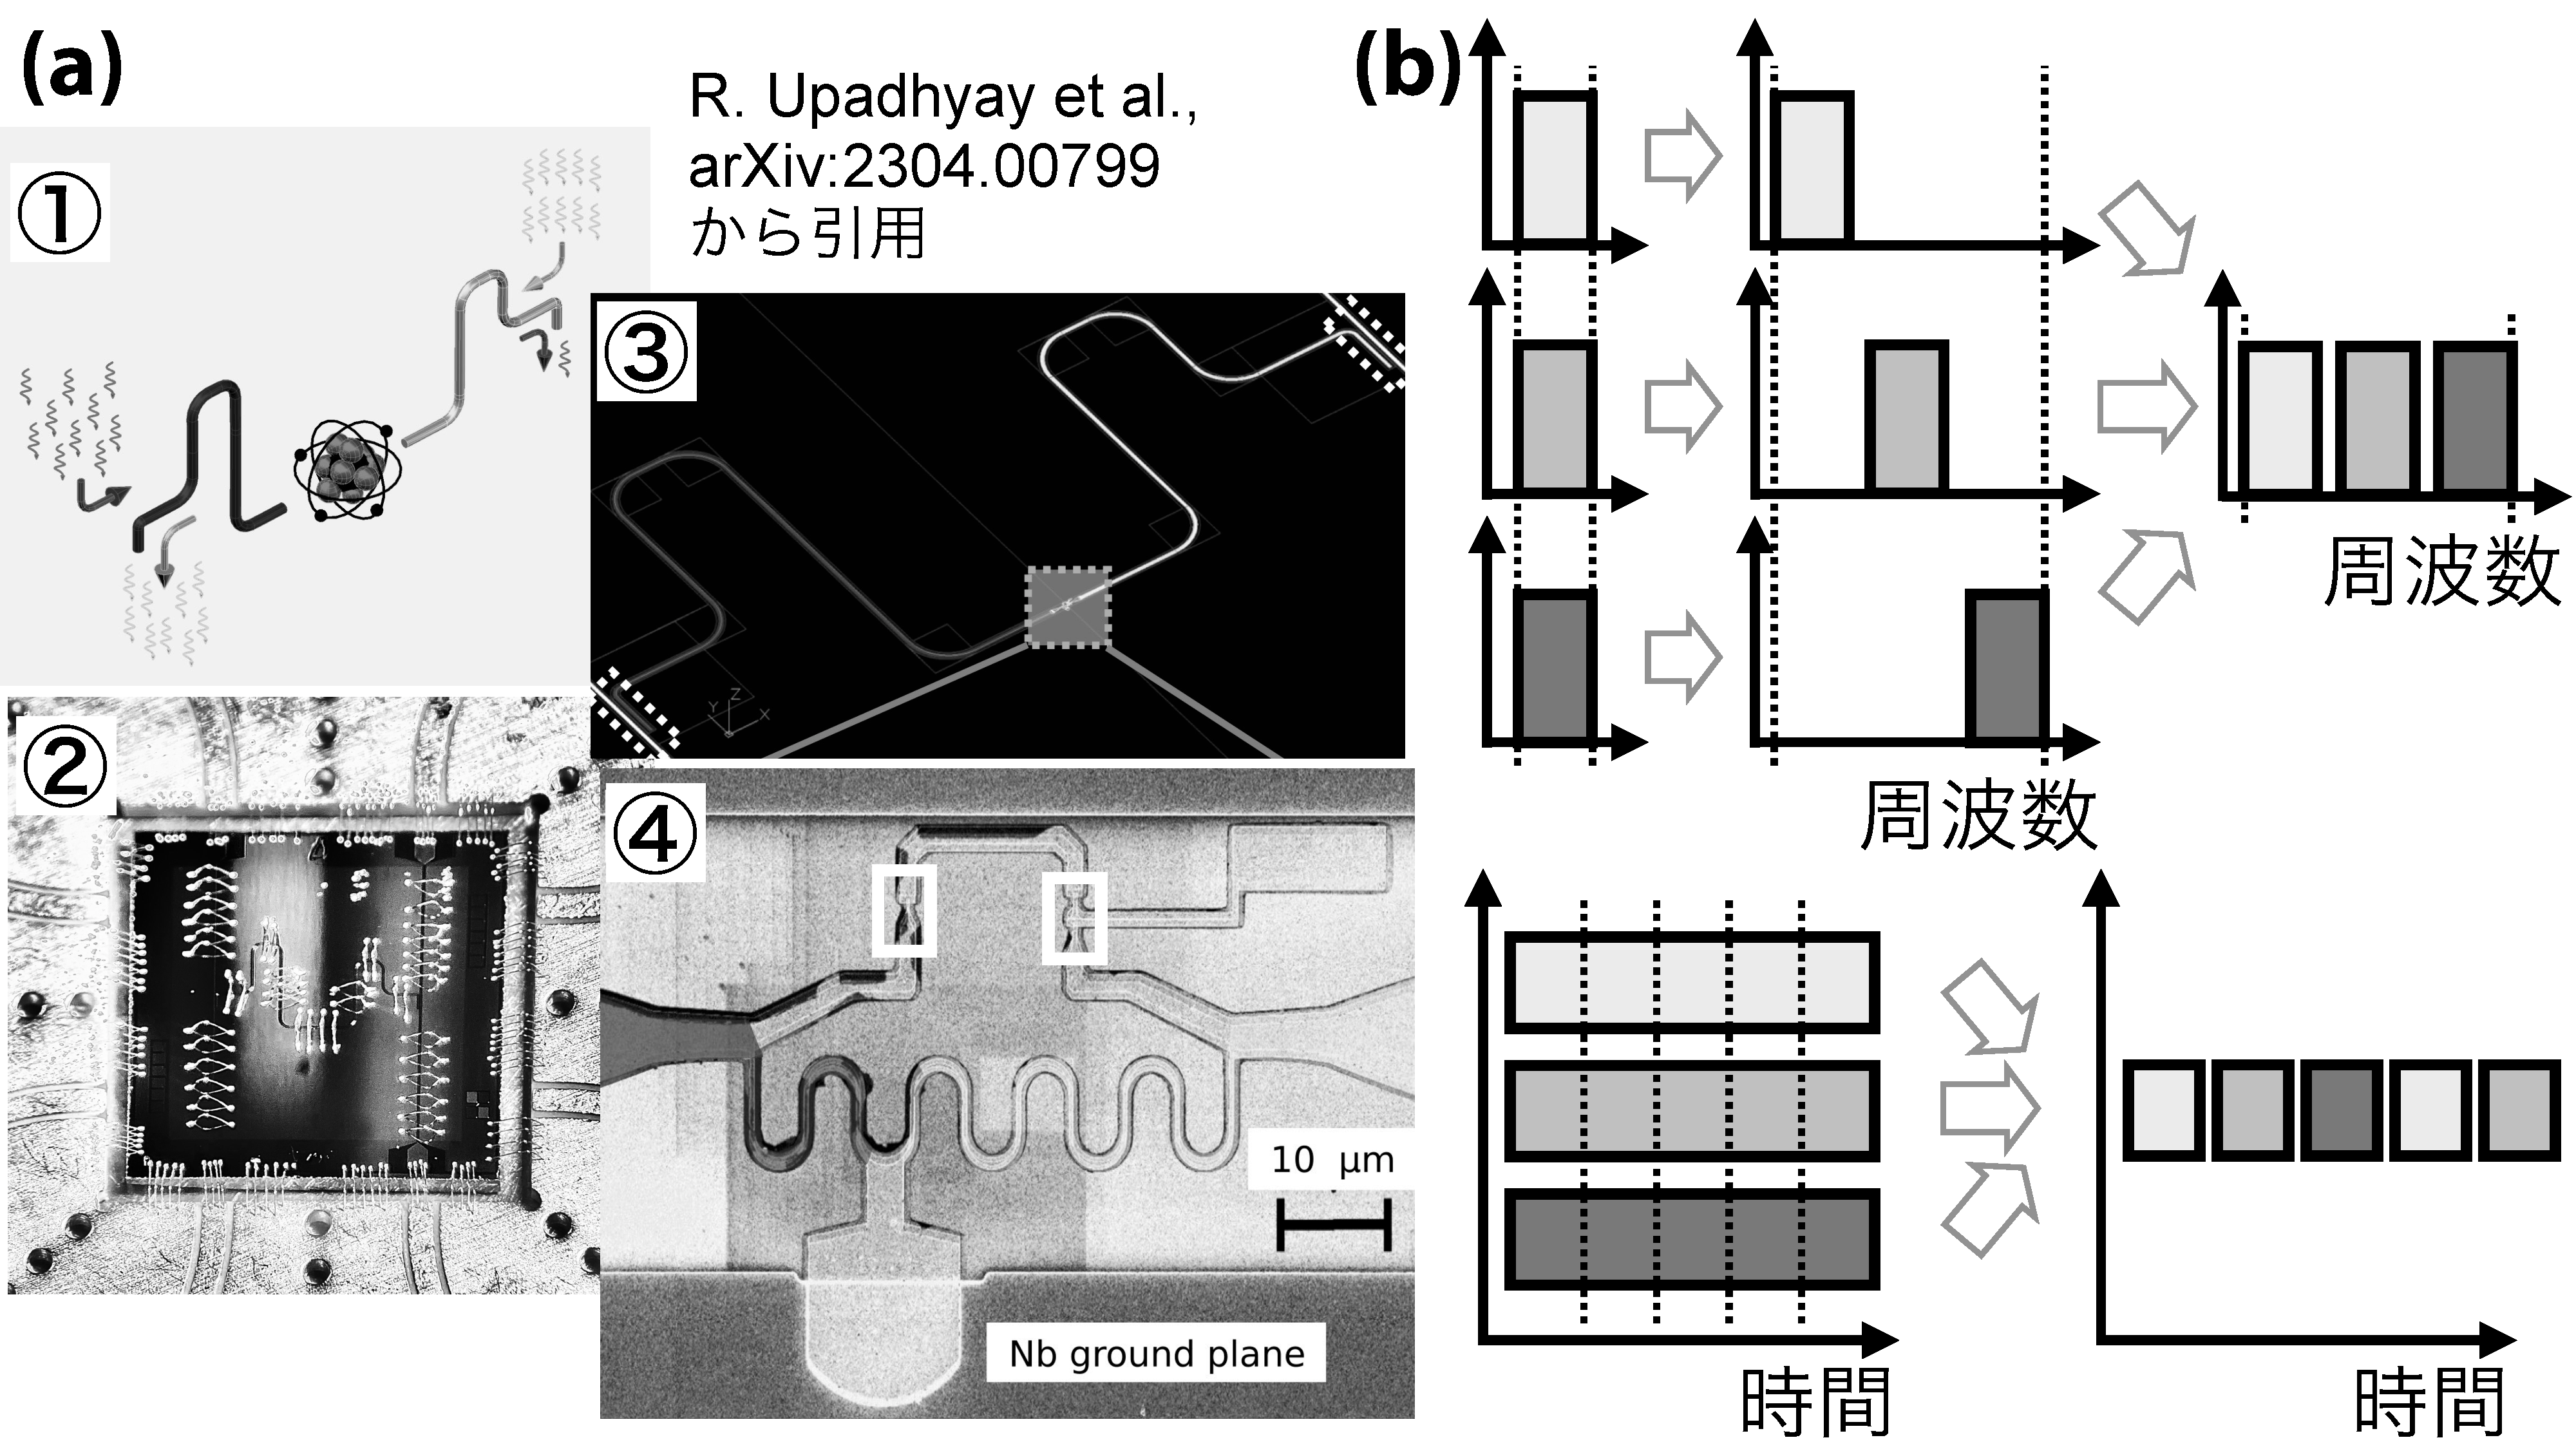
\includegraphics[width=10.5cm]{figs/hard}\vspace{-0.4cm}
		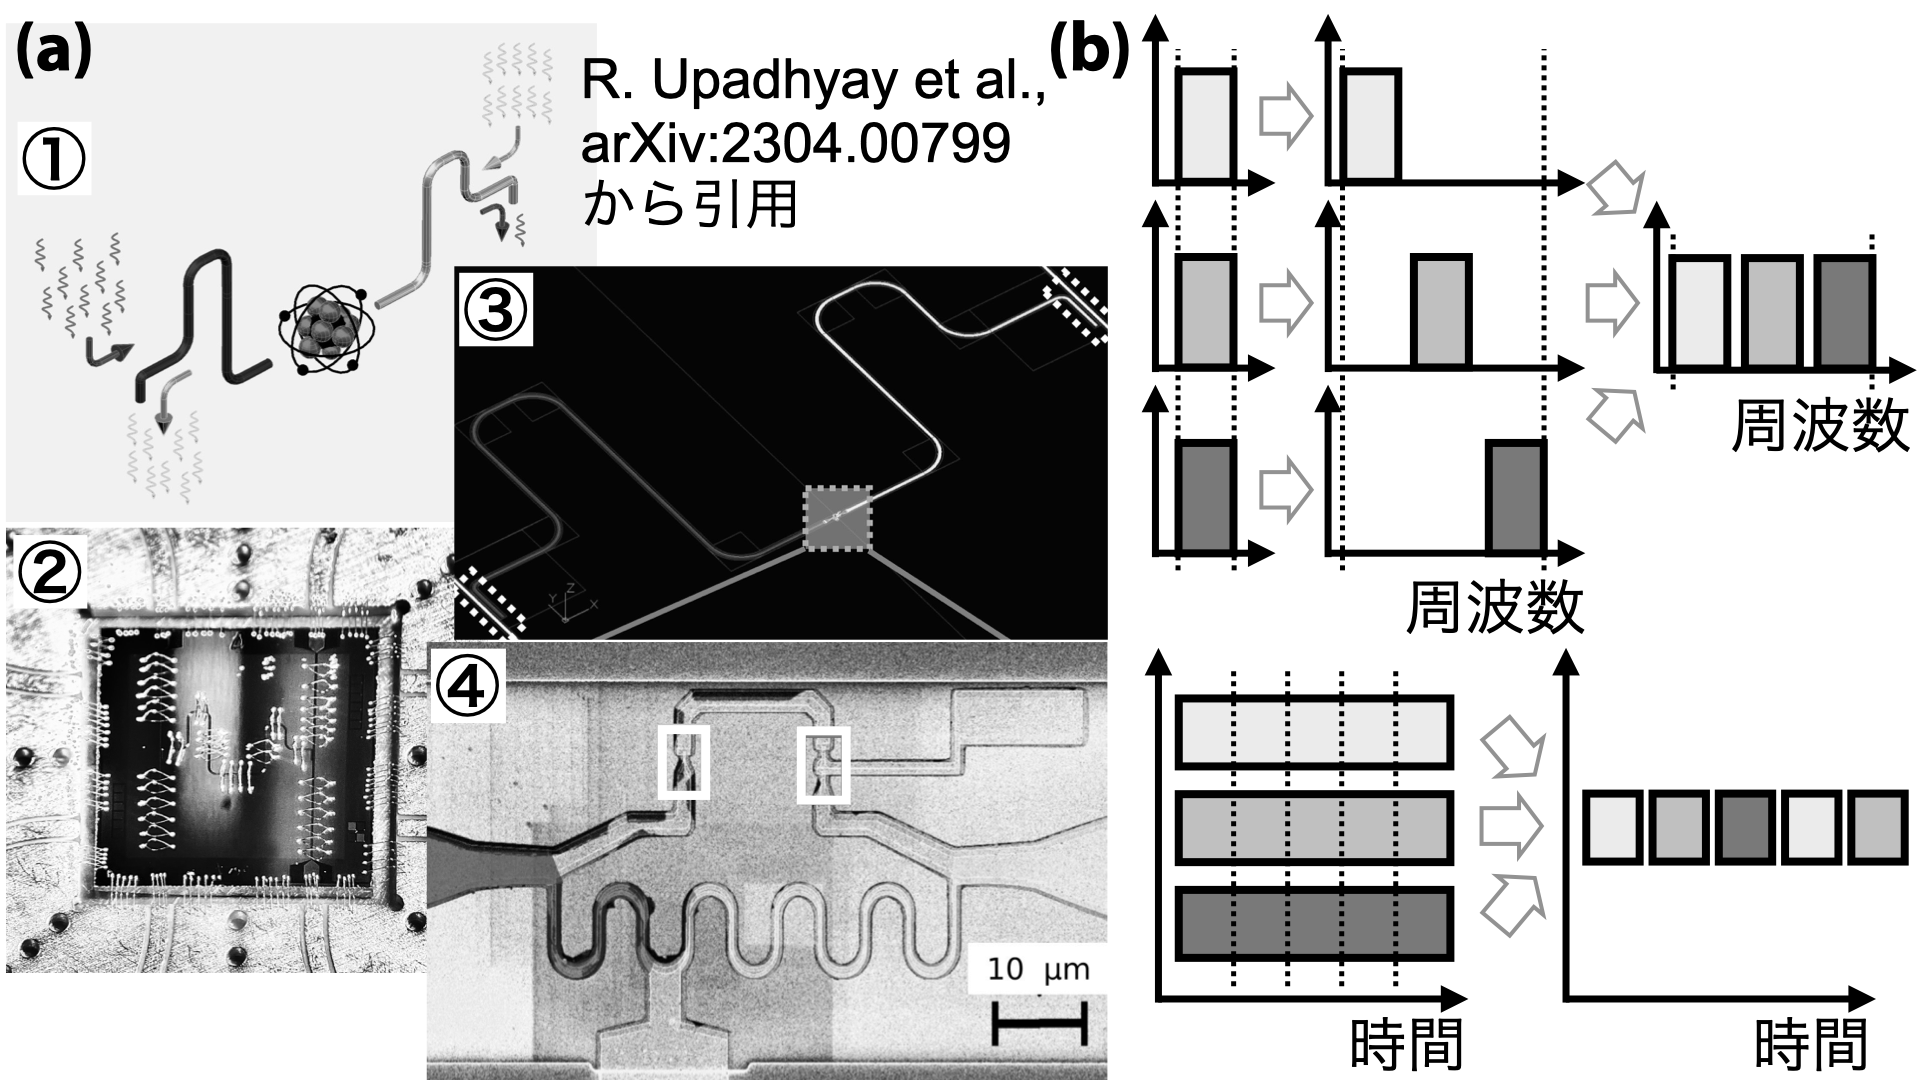
\includegraphics[width=10.8cm]{figs/hard.png}\vspace{-0.4cm}
		\caption{\small{(a)ジョセフソン接合ベースの整流素子([\ref{JJ_reciprocle}]から引用)。\maruone 一方向からの光だけを通しやすい性質を持つ。\marutwo 実際のデバイスの写真。\maruthree 3個のジョセフソン接合をもつ超伝導磁束量子ビット(中央の点線で囲まれた領域)と、左右に伸びる二つの共振器から構成される。\marufour 中央点線部分の拡大図。左の白四角に1個、右の白四角に2個のジョセフソン接合が作られている。(b)周波数分割の多重化(上)と時間分割の多重化(下)のイメージ。}
		\label{fig:hard}}\vspace{-0.7cm}
	\end{center}
\end{wrapfigure}

ハードウェア課題の着眼点はよりシンプルである。アイソレータやサーキュレータは高周波マイクロ波の整流を行う素子であり、超伝導量子コンピュータでは読み出しケーブルから逆流してきたノイズがアンプを通じて増幅されるのを阻止する重要な役割を果たす。通常これらは強磁性体の偏極に対して特定の方向にしか光を通さない性質(相反性)を利用しているが、偏極させるための永久磁石の磁場を閉じ込めるためのシールドが必要であり小型化のボトルネックとなっている。そこで近年強磁性体の代わりに\mybf{\ul{ジョセフソン接合の非線形光学効果を利用して相反性を実現}}する試みが提案され[\ref{JJ_Muller}]、研究が盛んになってきている。ジョセフソン接合は通常200~{nm}四方程度の薄膜で表面実装される\footnote{超伝導量子ビットを構成しているパーツの一つでもある。}ため小型化が容易で、かつ量子ビットと同じチップ上に載せることも原理的に可能である。既にハードウェアの実装例もあるが(図~\ref{fig:hard}(a))、まだ研究は初期段階にあり、相反性が小さいこと、挿入損失の大きいことなど課題は多く実用レベルにはない。これらを改善し、\mybf{\ul{従来型素子の性能に近づけるのが本研究の目的である。}}

一つの配線に信号を複数重畳させるチャネル多重化に関しては、周波数領域での多重化が既にIBMの実機などで実装されている。
量子ビットごとに固有周波数が違うことを利用し、異なる周波数のマイクロ波を重ねて処理・伝送するものだが(図~\ref{fig:hard}(b)上)、混線による制限があるため多重度は最大で8-10となっている。
一方で異なる量子ビットの信号を時間方向で分散させて同じ配線で送る時間領域の多重化(図~\ref{fig:hard}(b)下)はまだ報告されていない。
読み出しやゲート時間が多重度の分だけ長くなるデメリットがあるが、エラー訂正込みの量子演算における所要時間のボトルネックは古典計算機の処理時間だと考えられているため、ある程度のところまでは問題とならない\footnote{例えば(2)の冒頭で述べたパリティ計算は現在FPGAを用いても2~${\mu \mathrm{s}}$ほどはかかる。一方状態測定は現在最速の方法で150~ns、ゲート操作は典型的に10-100~nsである。}。従来の周波数領域での多重化とも同時に実装できるため、実現できた場合は大きな改善となる。\\


%また、以下のように本研究グループは\mybf{研究に必要なハードウェアとソフトウェアの技術}をすでに持っており、そのことも本研究を現実的なものにしている。
%
%\underline{\bf ハードウェア}\vspace{-2mm}
%\begin{itemize}
%\item ジョセフソン接合の製作に必要な微細加工の技術に精通し、それを用いた\mybf{超伝導量子素子の製作に成功}している。\vspace{-2mm}
%\item \mybf{希釈冷凍機に実装する環境を構築}し、コヒーレンス時間の測定など\mybf{量子ビットとしての性能評価を行う}ことができる。\vspace{-2mm}
%\item 長年取り組んでいる大型素粒子実験を通じ、\mybf{大量の読み出しチャンネルの時間制御技術を有している}。
%\end{itemize}

%\underline{\bf ソフトウェア}\vspace{-2mm}
%\begin{itemize}
%\item 素粒子物理の基本原理に精通しており、\mybf{対称性を量子回路に実装する技術}を持っている。\vspace{-2mm}
%\item エラー検知には物理量子ビットと補助量子ビット間で大量の2量子ビットゲートを使うが、その超伝導量子コンピュータでの実装に使われる\mybf{「交差共鳴パルス」のシミュレーションや最適なシークエンス設計に精通}している。
%\end{itemize}


%%%%%%%%%%%%%%%%%%%%%%%%%%%%%%%%%%%%%%
\noindent{\bf (4)何をどのように、どこまで明らかにしようとするのか}\\
%\begin{comment}
\begin{wrapfigure}{r}{6.5cm}
	\begin{center}
		\vspace{-1.3cm}
		%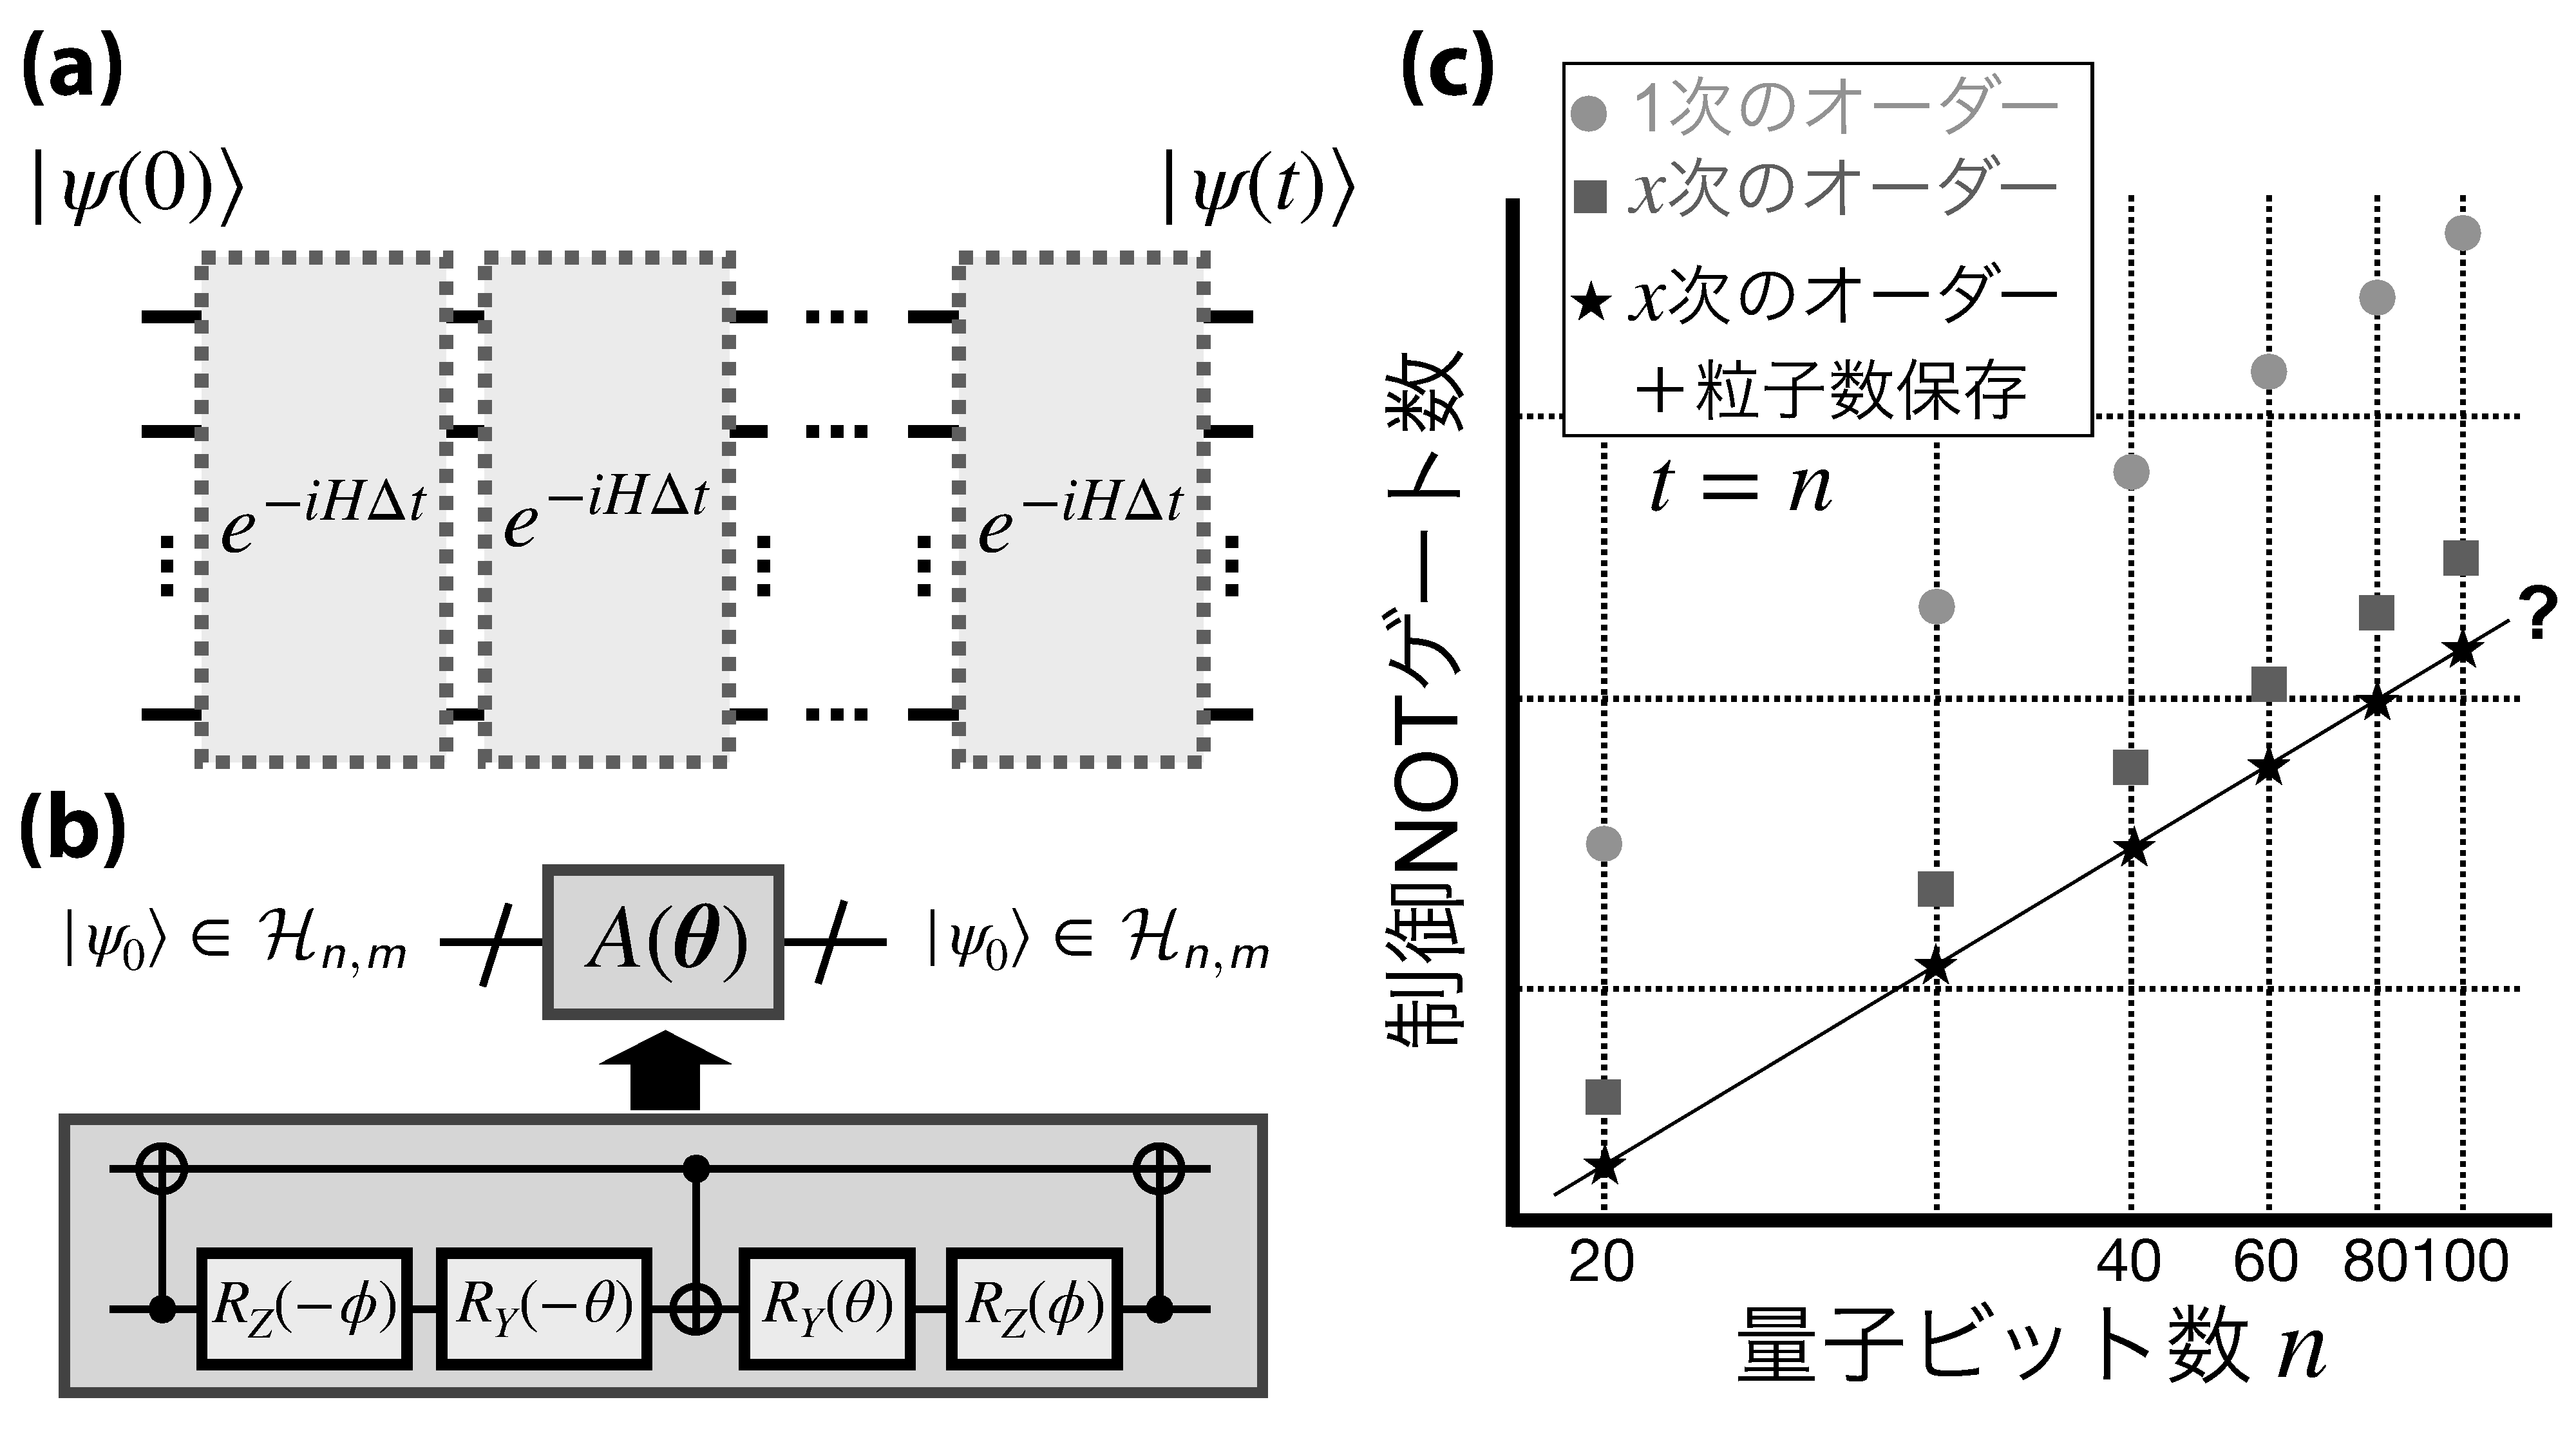
\includegraphics[width=10.5cm]{figs/trotter}\vspace{-0.4cm}
		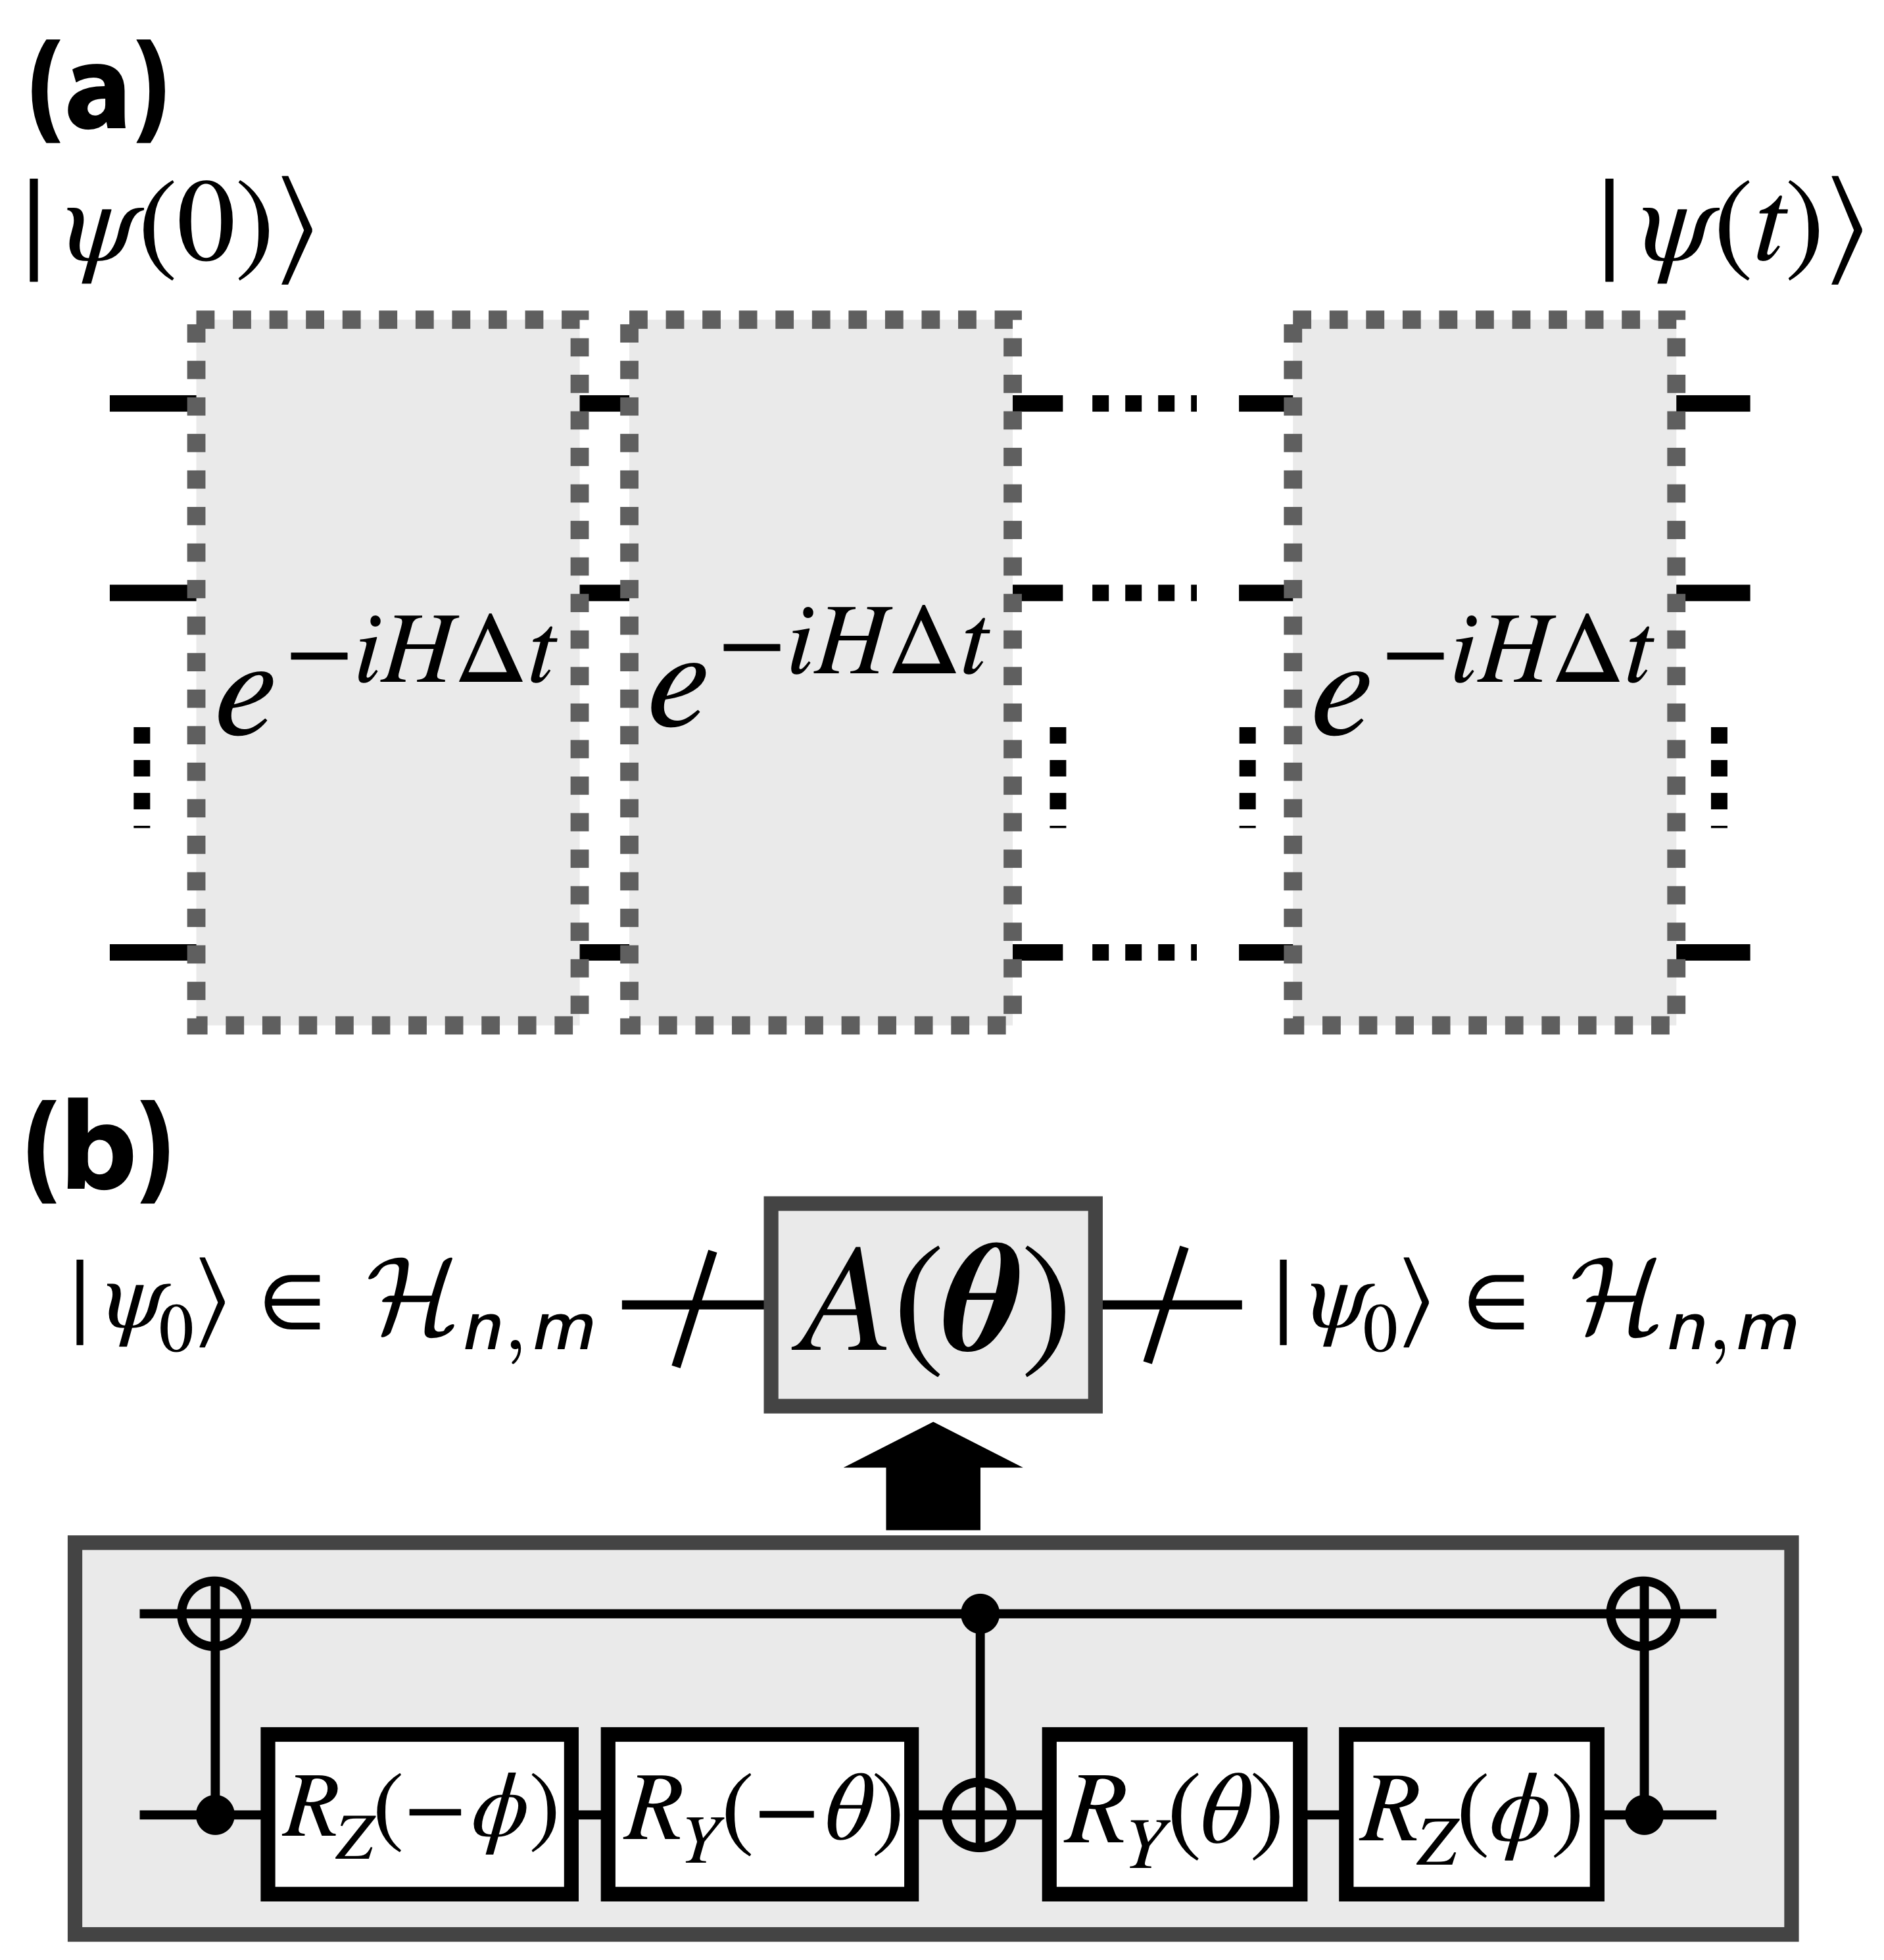
\includegraphics[width=5.5cm]{figs/trotter.png}\vspace{-0.4cm}
		\caption{\small{(a)ハミルトニアン時間発展$|\psi(t)\rangle=e^{-iHt}|\psi(0)\rangle$の鈴木-トロッター分解を用いた量子回路。(b)$n$量子ビット系で粒子数$m$を保存する量子回路(上)は2量子ビットゲート(下)で実装可能。%(c)誤差0.1\%でシミュレートするために必要な量子ビット数-制御NOTゲート数の関係を、鈴木-トロッター近似のオーダーと時間ステップを変えて評価する。
		}
		\label{fig:z2}}\vspace{-0.7cm}
	\end{center}
\end{wrapfigure}
%\end{comment}
\noindent \mybf{\ul{\maruone\ 2次元の格子ゲージ理論における対称性・保存量の量子ゲート表現}} \\
%
初期のFTQCでの優位性を示すことのできる問題として、素粒子物理を記述する\mybf{ゲージ理論の量子シミュレーション}を考える。特に\mybf{2次元の格子ゲージ理論($\pmb{U(1)}$ゲージ場を離散化した$\pmb{\mathbb{Z}_2}$ゲージ理論)}では、外部電場が存在する時に\mybf{物質が局所的な空間に閉じ込められる現象}が起こる。この現象を古典的にシミュレートするには、時間発展の各時間ステップごとに外部電荷の設定を変えて繰り返し計算する必要があるため、高い計算コストがかかる。量子シミュレーションは時間発展をより効率的に行えるため、量子コンピュータの優位性を示すことができる可能性がある。
量子計算では2次元$\mathbb{Z}_2$ゲージ場のハミルトニアンによる時間発展を、鈴木-トロッター分解(図~\ref{fig:z2}(a))を使ってユニタリー演算子の積に近似して実行する。
本研究の最初のステップは、\mybf{\ul{量子状態が保持する対称性(空間反転パリティ、粒子数)を取り入れた量子ゲートと一般的な量子ゲートを使って、時間発展した状態を量子回路に実装することである}}(図~\ref{fig:z2}(b))。
対称性を導入することで部分空間のみでの時間発展を考えることができるため、必要な量子ゲート数を削減できることが期待できる。この振る舞いを古典計算機のシミュレータで確認し評価を行う。逆に、これによって発生する冗長性を次項で述べるエラー訂正に利用できる。 \\
%シミュレータを使って時間発展シミュレーションを行い、時間発展状態のエネルギーや外部電場による閉じ込め効果を測定する。\vspace{-4mm}\\



%\underline{\bf マイルストーン}\vspace{-2mm}
%\begin{itemize}
%\item 20量子ビットの系に対して、特定の鈴木-トロッター近似のオーダー$\Omega$と時間ステップ$N$に対して、誤差1\%以下でのエネルギー測定を行う。\vspace{-2mm}
%\item $\Omega$と$N$を変え、誤差0.1\%以下でのシミュレーションに必要な2量子ビットゲート数を評価する。その評価結果を20量子ビット以上の系に対して外挿する(図~\ref{fig:z2}(c))。\vspace{-2mm}
%\item 対称性を取り入れた量子ゲートを使うことで、一般的な量子ゲートを使った場合の約半分の2量子ビットゲート数に抑えられることを示す(図~\ref{fig:z2}(c))。
%\end{itemize}
%
%
%%%%%%%%%%%%%%%%%%%%%%%%
\noindent \mybf{\ul{\marutwo\ 対称性を用いたエラー訂正手法の開発}} \\
%
量子ビットは状態操作や読み出しのために外部環境と相互作用しなければならないため、外的な要因によってエラーが起こることは避けがたい。ある対称性を持つ物理系を考える場合、その\mybf{保存量を繰り返し測定し途中で結果が変わった場合、測定の間でエラーが起こったと推定}できる。そのための典型的なエラー検知の方法はスタビライザー測定と呼ばれており、物理量子ビットでビット反転や位相反転が起こった時に、測定した補助量子ビットのパリティ検査の結果からエラーを検知する。
本研究では、2次元$\mathbb{Z}_2$ゲージ場での保存量として粒子数や空間反転パリティに着目し、それらの量を測定する対称オペレータを定義する。
閉じ込め効果など興味のある観測量の測定をしながら、対称性を保っているか(エラーが起こっていないか)判定するためには、\mybf{観測量と可換な対称オペレータを同時に測定}する必要がある。エラー緩和の先行研究をベースに、この同時測定のための手法を量子回路として実行する。
対称オペレータの測定結果が初期状態での予想量と一致していない場合に、対称性を回復させる(エラーを訂正する)ためのデコーダーを開発する。\vspace{-4mm}\\

\underline{\bf マイルストーン}\vspace{-2mm}
\begin{itemize}
\item 20量子ビットの系に対して、粒子数を対称オペレータ、時間発展状態のエネルギーを物理量として測定する量子回路を実装する。そこに10\%のエラーレートを持つ一般的な分極ノイズモデルを適用し、対称性によるエラー検知が可能であることを示す。\vspace{-2mm}
\item 初期状態の粒子数に誤差1\%で訂正するためのユニタリー演算子を機械学習モデルを使って決定する(デコーダーの開発)。\vspace{-2mm}
\item 量子コンピュータの実機を使って検証実験を行い、エネルギー測定の精度がエラー訂正によって向上することを確認する。
\end{itemize}


%%%%%%%%%%%%%%%%%%%%%%%%
\noindent \mybf{\ul{\maruthree\ ジョセフソン接合を用いた低損失オンチップ小型サーキュレータ/アイソレータの開発}} \\
ジョセフソン接合ベースで現在最高の性能を出しているサーキュレータは相反度(in/outポートの順流・逆流でのマイクロ波透過率の比)が3dB・挿入損失(順流におけるマイクロ波透過率)が10dBとなっており[\ref{JJ_circulator}]、強磁性体ベースのサーキュレータが典型的に相反度40dB・挿入損失2dBほどであることを考えると、まだ実用には程遠い。
理論上15dBほどの相反度が単体で見込めるとされているが[\ref{JJ_Muller}]、実現のために複数あるジョセフソン接合の抵抗値を0.1\%のオーダーで揃える必要があると言われており[\ref{JJ_circulator}]、技術上不可能ではないものの相当な開発を要する。一方で、微細化することのメリットの一つとして素子を直列に繋ぐことで性能を倍増させられるというものがある。挿入損失も倍増するが、こちらはまだ回路のデザイン次第で改善の余地が大きく、より現実的である。\vspace{1mm}

\underline{\bf マイルストーン} \vspace{-1mm}
\begin{itemize}
\item 単体で相反度5dB・挿入損失1dBの低損失素子を実現する。\vspace{-2mm}
\item 直列に並べたサーキュレータを量子チップと同じチップに実装する。%\vspace{1mm}
\end{itemize}

%%%%%%%%%%%%%%%%%%%%%%%%
\noindent \mybf{\ul{\marufour\ 超伝導量子コンピューター配線の時間領域多重化}} \\
\vspace{-4mm}\\
量子ビットのゲート操作と状態測定ともにマイクロ波の照射によって行われるが、本研究ではよりシンプルな状態測定に集中する。
量子ビットの状態の測定は、同じチップ上で量子ビットと結合した平面導波管にマイクロ波パルスを透過させた際の位相を測定することによって行われる。
高周波回路では導波管は共振器としての性質を持つが、この共振周波数が結合した量子ビットの状態によって変わることを利用している。
このときのマイクロ波パルスの長さが現状最短で150~nsである[\ref{fastReadout}]。測定パルスの到達時間をすらして各量子ビットを区別する時間領域の多重化では、各々のパルス長が多重度の上限を決めることとなる。量子ビットと導波管の結合を強めることでこのパルスを短縮することができる。通常これは量子ビットとノイズの相互作用も増やすため短寿命化をもたらすが、量子演算を行う物理ビットが長い寿命(100~$\mu \mathrm{s}$)を要求するのに対し、エラー訂正用の補助量子ビットは各演算操作ごとにリセットさせるためゲート間隔(1~$\mu \mathrm{s}$)ほどの寿命で十分である。またマイクロ波パルスの間隔も、ジッターを制御することで10~ns以下にすることが可能である。これらの技術を組み合わせることで、現在の技術で達成できる最大限の多重化を目指す。\vspace{1mm}

\underline{\bf マイルストーン} \vspace{-1mm}
\begin{itemize}
\item 読み出し用導波管と強結合させた量子ビットを使って、測定精度99\%以上を維持しながら100~nsを切る測定時間を実現する。\vspace{-2mm}
\item 状態測定の時間を全体で1~${\mu \mathrm{s}}$に収めながら5倍の多重化を達成する。 
\end{itemize}


%%%%%%%%%%%%%%%%%%%%%%%%
\noindent{\bf (5)目的を達成するための準備状況}\\
最初のステップである物理問題の設定については、本研究に先行して、1次元$U(1)$ゲージ理論である\mybf{シュウィンガー模型}のシミュレーションに取り組んできた。シュウィンガー模型はシンプルでありながら、カイラル対称性(粒子のスピンの向きに関する変換対称性)の破れなど、現実世界の非可換ゲージ理論と同じ性質を共有しており、場の理論のシミュレーションではベンチマークとして良く活用される。本研究グループは、\mybf{シュウィンガー模型でのエネルギー基底状態やその時間発展状態を近似する状態を、パラメータ化した量子回路を使って量子コンピュータに実装する}研究を進めてきた。基底状態については変分量子固有値ソルバー、時間発展状態については時間依存変分量子シミュレーションと呼ばれる手法を使ってシミュレーションを行っている。\mybf{1次元$\pmb{\mathbb{Z}_2}$ゲージ理論のハミルトニアン時間発展を鈴木-トロッター分解の方法を使ってシミュレーションを行い、その状態が\ul{電場の有無によって閉じ込め相と非閉じ込め相に別れていくことなどを確認}}した(図~\ref{fig:status}(a))~[\ref{Terashi_QML_Qdata}]。
物理系が持つ対称性を考慮した量子回路の設計は、本研究の重要なステップである。本研究グループはシュウィンガー模型の時間発展シミュレーションの研究の中で、\mybf{粒子数を保存する量子ゲートを実装した回路を使って\ul{長時間の時間発展シミュレーションを行うことに成功}}している。対称性を持つ量子回路が張るヒルベルト空間は全空間の一部に限定されるため、量子回路のパラメータ決定を効率良く行うことができる。この手法を$\mathbb{Z}_2$ゲージ理論のシミュレーションに応用することは比較的容易である。

\begin{wrapfigure}{r}{11cm}
	\begin{center}
		\vspace{-0.8cm}
		%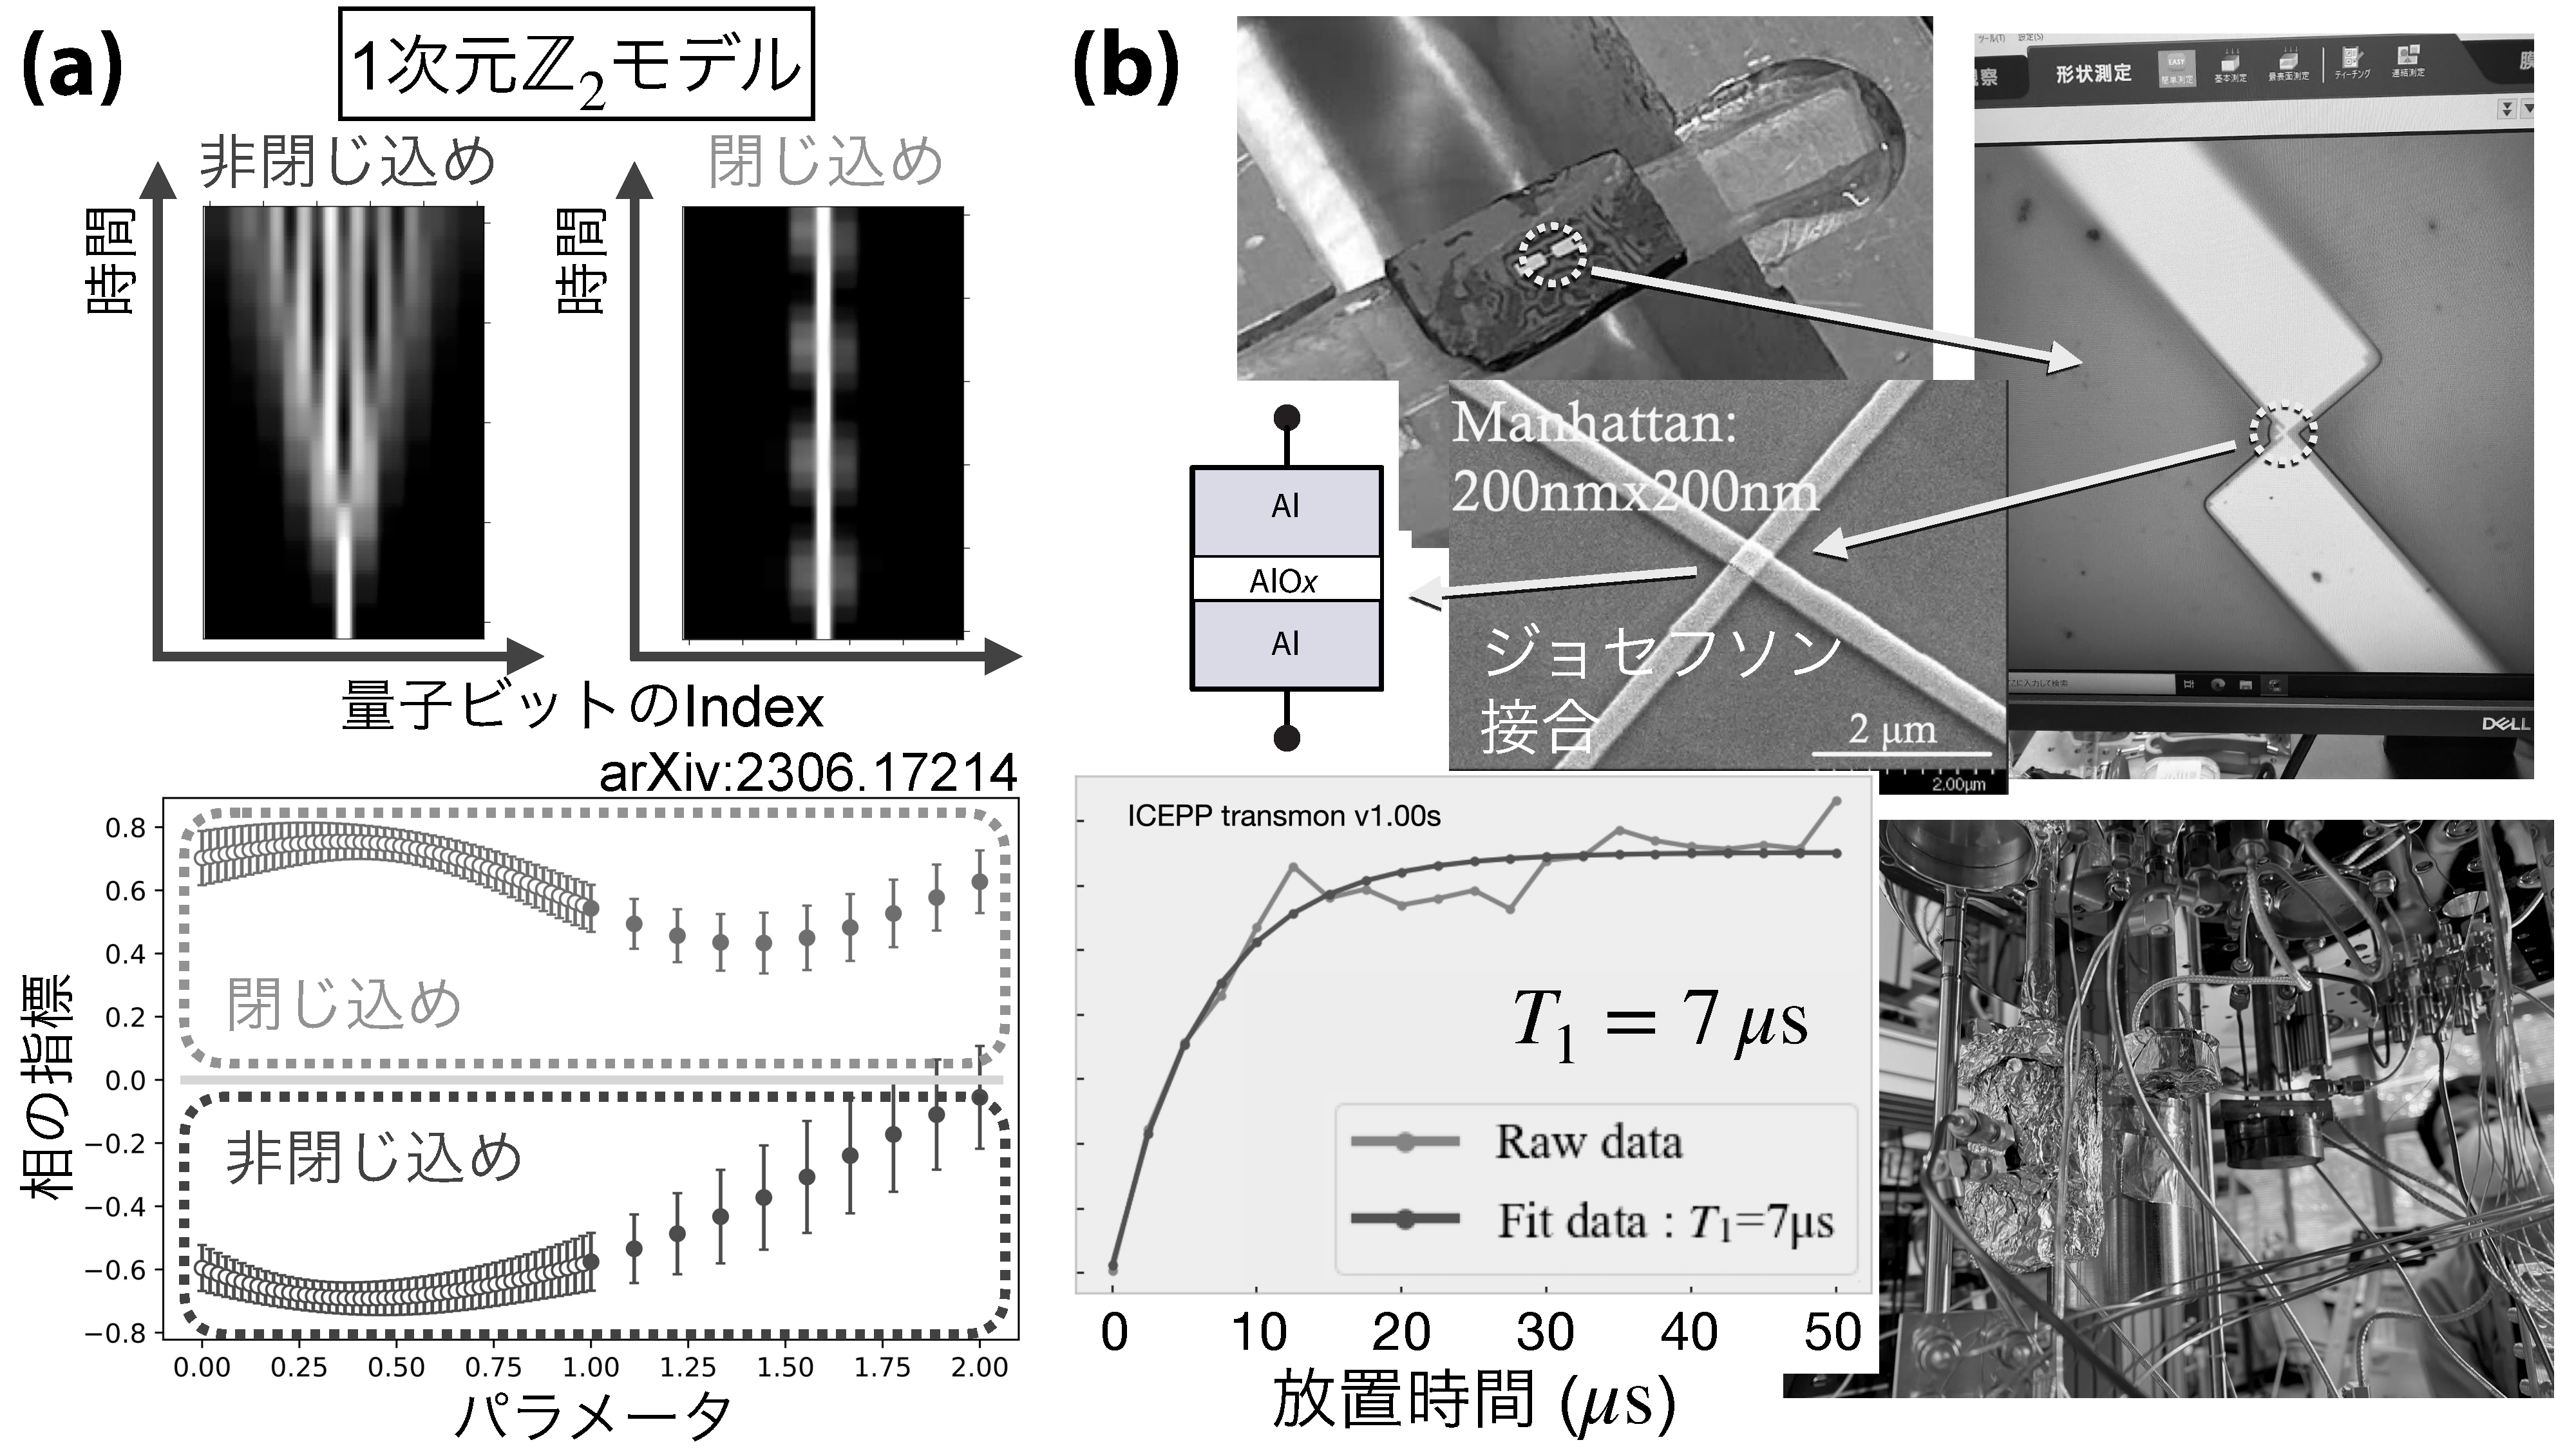
\includegraphics[width=11cm]{figs/result}\vspace{-0.3cm}
		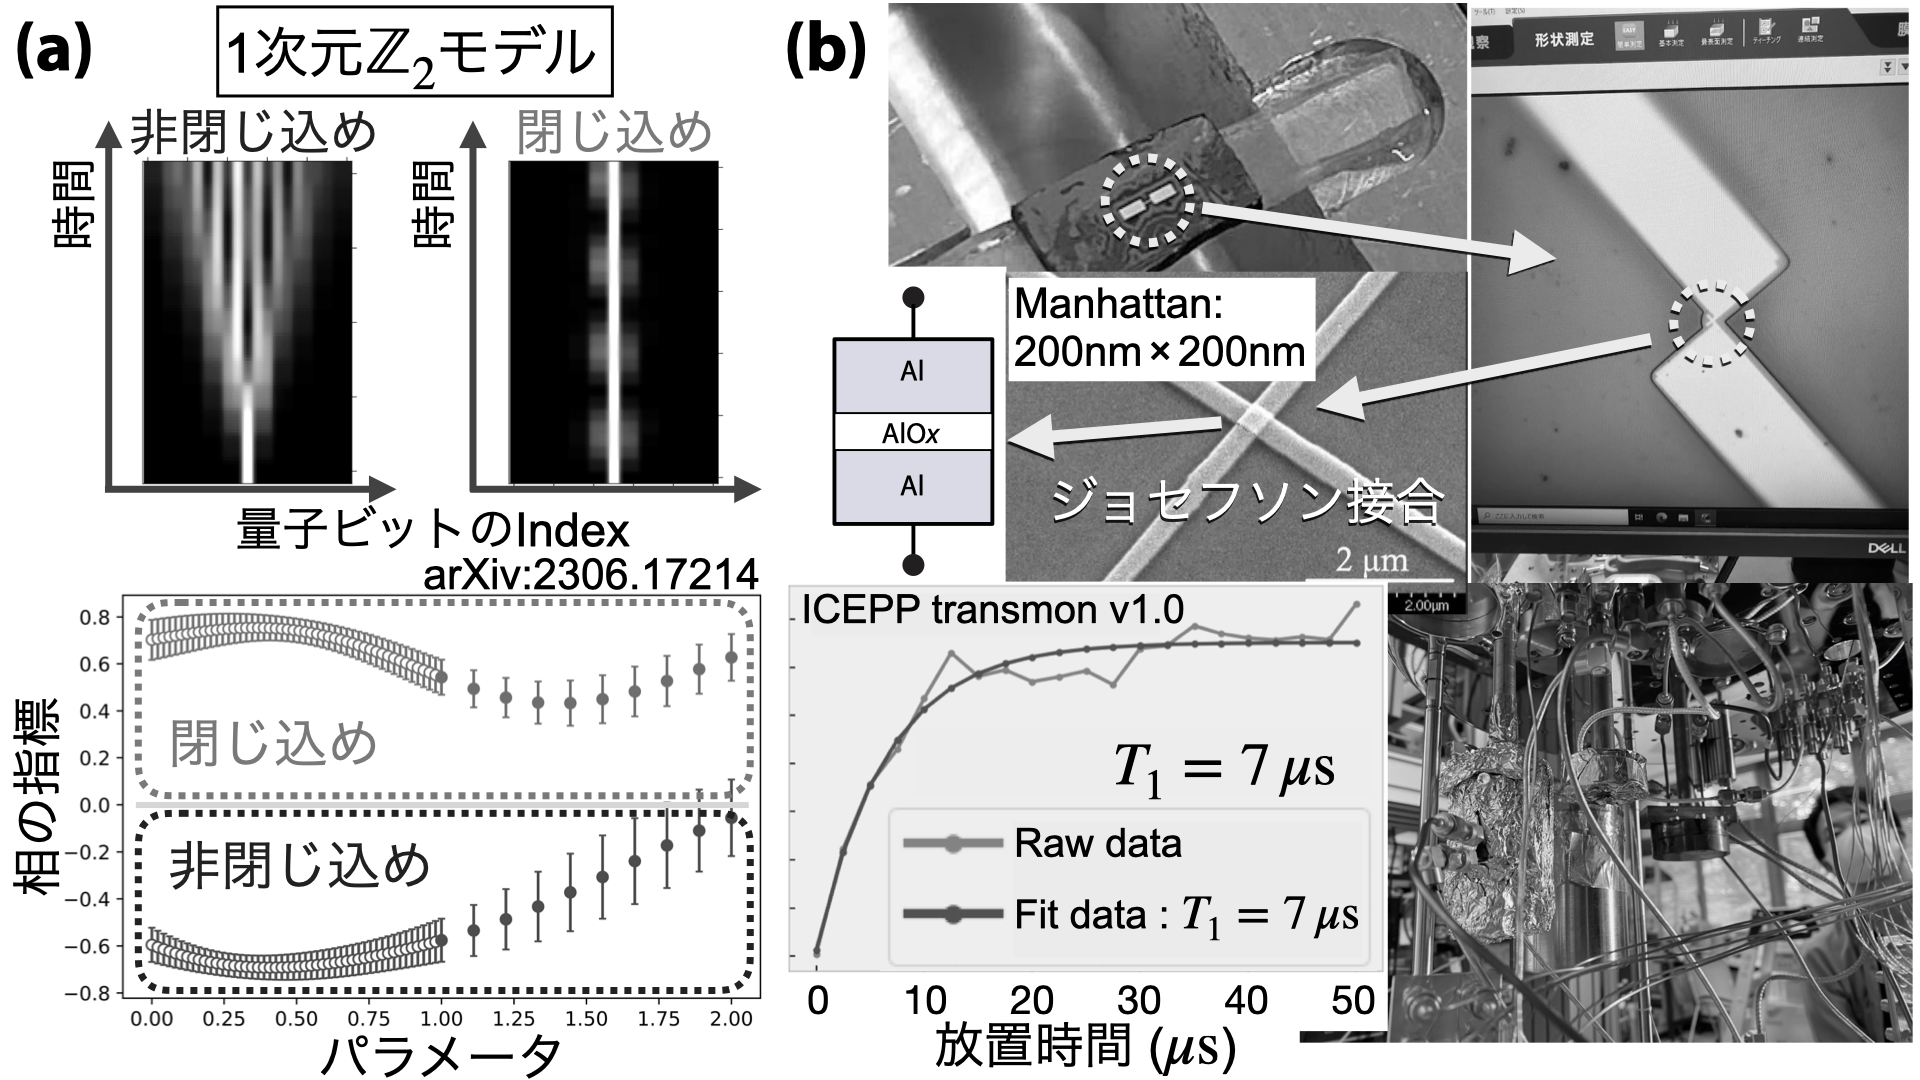
\includegraphics[width=11cm]{figs/result.png}\vspace{-0.4cm}
		\caption{\small{(a)1次元$\mathbb{Z}_2$ゲージ理論で、物質場が時間発展と共に拡散していく様子(非閉じ込め, 左)。右は拡散しない場合(閉じ込め)。鈴木-トロッター分解を用いた量子回路で時間発展状態をシミュレートし、閉じ込め相と非閉じ込め相の相分類を行った(下)~[\ref{Terashi_QML_Qdata}]。(b)本研究グループによって製作された超伝導量子ビットの写真。中央の$200~{\rm nm}\times200~{\rm nm}$の領域にジョセフソン接合がある。低温科学センターにある希釈冷凍機(右下)と、製作した超伝導量子ビットが$|1\rangle$状態から$|0\rangle$に脱励起するまでの時間($T_1$)の測定結果(左下)。$T_1=7~\mu{\rm s}$を達成している。}
		\label{fig:status}}\vspace{-1cm}
	\end{center}
\end{wrapfigure}

ハードウェア開発には、ジョセフソン接合を含めた超伝導量子素子の製作に必要な\mybf{微細加工技術の習得}と\mybf{希釈冷凍機・マイクロ波制御のエレクトロニクスなどからなるテスト環境の整備}が一通り達成されている。現在\mybf{10~$\boldsymbol{\mu}$s程度の寿命を持つ\ul{超伝導量子ビット}}は1日半ほどの製作時間で再現性よく作ることに成功している(図~\ref{fig:status}(b))。これは本研究の開発に要求される水準を十分にクリアしている。 \vspace{-3mm}\\


\noindent{\bf 研究者の役割}\\
研究協力者であるポスドク研究者・大学院生とともに、研究代表者が研究課題{\maruone}を担当する。課題{\marutwo}については、古典計算ソフトウェアと超伝導量子ビットの物理シミュレーションの知識が豊富である研究分担者(飯山)が主導して進める。課題{\maruthree}{\marufour}については、超伝導量子素子の製作に成功し、マイクロ波のエンジニアリング技術にも精通する研究分担者(陳)が中心となって進める。


\vspace*{0.5zw}
\noindent\textbf{参考文献} \vspace{-2mm}
\begin{enumerate}
	\renewcommand{\labelenumi}{[\arabic{enumi}]}

	\item \label{errorRateBenchmark} %``Quantum logic with spin qubits crossing the surface code threshold"
		X.~Xue {\it et al.}, {\it Nature} {\bf 601}, 343 (2022).\vspace{-3mm}
	\item \label{fastReadout} %``Transmon qubit readout fidelity at the threshold for quantum error correction without a quantum-limited amplifier" 
		Y.~Kim {\it et al.}, {\it npj Quantum Information} {\bf 9}, 26 (2023).\vspace{-3mm}
	\item \label{IBM_Utility} %``Evidence for the utility of quantum computing before fault tolerance'',
		Y.~Kim {\it et al.}, {\it Nature} {\bf 618}, 500 (2023).\vspace{-3mm}
	\item \label{Google} %``Suppressing quantum errors by scaling a surface code logical qubit'', 
		Google Quantum AI, {\it Nature} {\bf 614}, 676 (2023).\vspace{-3mm}
	\item \label{LDPC2} %``Constant-Overhead Quantum Error Correction with Thin Planar Connectivity'', 
		M.~A.~Tremblay {\it et al.}, {\it Phys. Rev. Lett.} {\bf 129}, 050504 (2022).\vspace{-3mm}
	%\item \label{AQCEL} ``Quantum Gate Pattern Recognition and Circuit Optimization for Scientific Applications'',
	% 	W.~Jang, \me {\it et al.}, arXiv:2102.10008 (2021).\vspace{-3mm}
	%\item \label{NTT} ``Cryogenic operation of NanoBridge at 4 K for controlling qubit'', 
	%	K.~Okamoto {\it et al.}, Jpn. J. Appl. Phys. {\bf 61}, SC1049 (2022).\vspace{-3mm}
	%\item \label{Pulse} ``Josephson Microwave Sources Applied to Quantum Information Systems'',
	%	A.~J.~Sirois {\it et al.}, {\it IEEE Transactions on Quantum Engineering}, {\bf 1}, 1 (2020).\vspace{-3mm}
	%\item \label{Passive} ``Two-resonator circuit quantum electrodynamics: A superconducting quantum switch'', 
	%	M.~Mariantoni {\it et al.}, {\it Phys. Rev. B} {\bf 78}, 104508 (2008).\vspace{-3mm}
	\item \label{JJ_Muller} %``Passive On-Chip Superconducting Circulator Using a Ring of Tunnel Junctions"
		C.~Muller {\it et al.}, {\it Phys. Rev. Lett.} {\bf 120}, 213602 (2018).\vspace{-3mm}
        \item \label{JJ_circulator} %``Passive Superconducting Circulator on a Chip'',
		R.~Navarathna {\it et al.}, {\it Phys. Rev. Lett.} {\bf 130}, 037001 (2023).\vspace{-3mm}
        \item \label{JJ_reciprocle} %``Microwave quantum diode'',
                R.~Upadhyay {\it et al.}, arXiv:2304.00799.\vspace{-3mm}
		
\end{enumerate}

%end 研究目的と研究計画	====================

% p01_purpose_plan_01.tex
\KLEndSubject{F}


%#Split: 02_abilities  
%#PieceName: p02_abilities
% p02_abilities_00.tex
\KLBeginSubject{02}{2}{2 応募者の研究遂行能力及び研究環境}{2}{F}{}{jsps-subject-header}{jsps-default-header}

\section{2 応募者の研究遂行能力及び研究環境}
%    <<最大 2ページ>>

% s14_abilities
%\PapersInstructions		% <-- 留意事項。これは消すか、コメントアウトしてください。
%begin 応募者の研究遂行能力及び研究環境 ====================
\noindent{\bf (1)これまでの研究活動}\\
応募者は欧州原子核研究機構(CERN)にある大型ハドロン加速器(LHC)を用いた大型実験ATLASに参画し、高エネルギー素粒子実験を最先端の現場で主導してきた。\mybf{ATLAS検出器のデータ取得システムの構築・運転から物理データ解析、次世代加速器実験への増強計画}まで豊富な知識と経験を有しており、それらの技術をもとに\mybf{量子コンピュータのアルゴリズム開発、量子シミュレーション、量子ソフトウェアとハードウェアの開発}を進めている。\vspace{-2mm}\\

高エネルギー素粒子実験への応用に向け、研究代表者(寺師)は2019年初頭から量子コンピュータの研究を開始した。カナダD-Wave社の量子アニーリングマシンを使い、組み合わせ最適化問題として検出器信号から測定した粒子の飛跡を再構成する研究に、米国ローレンスバークレー国立研究所の研究者とともに取り組んだ。この種の取り組みとしては世界的に最初期のものであり、量子アニーリングによって高い再構成効率が実現できることを示した~[\ref{Saito_CHEP}]。
その後、\mybf{\ul{パラメータ化した量子回路を用いてデータの関連性を学習する「量子機械学習」の手法を素粒子実験のデータ解析に取り入れ、比較的少数のデータや学習パラメータで古典機械学習手法に匹敵する学習性能を持ちうることを示した}}~[\ref{Terashi_QML_selection}]。量子機械学習で古典データを学習する場合、まずデータを量子状態に符号化し、その状態をパラメータ化した量子回路で変換し測定する。教師あり学習では、その測定結果がデータの教師ラベルに合うようにパラメータを最適化する。量子機械学習は\mybf{量子状態への符号化や学習回路の設計によっては学習が困難になる}ことが知られており(\mybf{勾配消失問題})、その解消に向けた研究を現在進めている。
また本研究課題に先行して、研究課題{\maruone}{\marutwo}に必要な場の理論の量子多体系シミュレーションにも取り組んできた。ポスドク研究者と共に、\mybf{\ul{シンプルな1次元シュウィンガー模型での基底状態}}や\underline{\mybf{$\pmb{\mathbb{Z}_2}$ゲージ理論の時間発展状態のシミュレーション}}に取り組み、\mybf{\ul{生成された状態が期待される性質やエネルギーを持つことを確認}}した。ここで生成したシミュレーションデータを使って、\mybf{IBMチューリッヒの研究者とともに量子状態(波動関数)から物理系の性質を直接学習する量子機械学習の応用}に取り組んだ~[\ref{Terashi_QML_Qdata}]。ここではデータの符号化が必要ではなく、かつ古典畳み込みニューラルネットワーク(CNN)に着想を得た\mybf{量子CNN}を学習回路として使うことで、勾配消失問題に強い学習が可能である。この学習モデルを使い、\mybf{\ul{シュウィンガー模型ではカイラル対称性の破れ}}、\underline{\mybf{$\pmb{\mathbb{Z}_2}$ゲージ理論では外部電場による物質場の閉じ込め}}に由来する\mybf{\ul{相転移のシミュレーションに成功}}した~[\ref{Terashi_QML_Qdata}]。

NISQコンピュータでは、ノイズの影響を抑えるためにユニタリー演算をより少ない量子ゲートを使って実装することが望ましい。超伝導量子コンピュータでは、特に制御NOTゲートのエラーレートが1\%程度と高く、主要なエラー源である。本研究グループは回路に現れる制御NOTゲートごとに量子状態を測定し、得られる計算基底の出現頻度から不要な制御NOTゲートを削減する最適化ツール\mybf{AQCEL}を開発した~[\ref{Terashi_AQCEL}]。AQCELを使い、\mybf{\ul{計算精度を落とすことなく場の理論のシミュレーション回路に現れる制御NOTゲートを75\%程度削減できることを実証}}した~[\ref{Terashi_AQCEL}]。

研究分担者(飯山)は、CERN LHCのもう一つの大型実験であるCMS実験において、数十ペタバイトにも及ぶ実験データを管理するソフトウェアの構築、実装を行うなど、科学計算やソフトウェア開発に関する経験を多く有している~[\ref{Iiyama_Dynamo}]。また、\mybf{機械学習技術、特にFPGAなど低レイテンシ環境でのアルゴリズム実行に関して、第一線での研究実績がある}~[\ref{Iiyama_GNN}]。2020年から量子コンピューティング研究に携わり、素粒子物理学への応用を念頭においた\mybf{\ul{量子状態生成アルゴリズムの考案}}や、\mybf{\ul{超伝導型量子ビットに代表される非調和振動子の物理シミュレーションの開発}}などを行ってきた。

研究分担者(陳)は、LHC-ATLAS実験において検出機の大規模データ取得システムの構築と運用に取り組んだ豊富な経験がある。25~ns毎に発生する陽子衝突を記録し、数十万以上の検出器チャンネルを正しいタイミングで帯域を逼迫させることなく後段に送るという非常にシビアな要件であるが、それを満たすための開発や運用を通じて、\mybf{\ul{高周波信号の時間制御やデータ圧縮・多重化に関する高いノウハウを有している。}}また2022年1月より量子コンピューターのハードウェア開発研究に携わっているが、表面微細加工技術の習得とともに、測定系の立ち上げも同センターの稲田聡明助教・新田龍海特任助教とともに主導し、\mybf{\ul{1年のうちに実用に耐える超伝導量子ビットの製作とその性能評価に成功している}} (図~\ref{fig:hard}(b))。また、量子力学基礎論の理論研究~[\ref{Chen_QM}]や超伝導量子ビットを用いた暗黒物質の探索手法の提案~[\ref{Chen_DM}]など、基礎物理と量子効果、量子計測技術などに対しても鋭い感覚を有している。\vspace{-2mm}\\


\noindent{\bf (2)研究環境}\\
本研究でのソフトウェア研究は、東京大学素粒子物理国際研究センターで運用する計算機システムを使って、量子多体系シミュレーションやアルゴリズムの開発を行う。量子ビット数とともに状態ベクトル空間は指数的に増大するため、量子系の古典計算機シミュレーションには大容量メモリが必要になる。本研究グループでは、すでに\mybf{\ul{テラバイトスケールのメモリと高性能GPGPUを搭載する計算機を複数台運用}}しており、\mybf{\ul{シミュレータとして格子ゲージ理論の量子シミュレーションや量子機械学習を行うことが可能}}である。本研究では、エラー訂正のための演算を決定するデコーダー用アルゴリズムの開発や、一般的な回路ノイズモデルに対するシミュレータでの性能検証が重要であり、そのためこの計算機環境をさらに拡張する。

ハードウェアに関しても開発に必要な環境は概ね整備できている。超伝導量子デバイスは東京大学武田先端知スーパークリーンルームおよび沖縄科学技術大学院大学 (OIST)の共同利用装置を用いて、電子線リソグラフィーや斜め蒸着・現像・エッチングを含めて1日半ほどで製作が可能である。測定は東京大学低温科学研究センターにて2022年4月より低温科学センター・極低温プラットフォームの共同利用装置群を立ち上げ、希釈冷凍機を用いた低温環境での量子ビットや量子アンプの安定した測定に成功している。\mybf{\ul{現在同時に10量子ビット程度を同時に測定できる環境が既に確立されている}}が、本研究で多重化の研究を新たにするにあたってより多ビットを同時測定できるよう、高周波回路素子、特に低温アンプや量子アンプなどを追加する予定である。
%またセンターで奥村恭幸准教授・石野雅也教授などのにはLHC-ATLAS実験におけるミューオン検出器で全検出器中最も困難な高周波信号処理 (30万チャネルの信号を数${\mu \mathrm{s}}$のレイテンシでFPGA処理) を実現してきたエキスパートである
%共振空洞に関しても東京大学理学部物理学科の試作室技術職員の大塚茂巳氏の指導の下、10~mKで無負荷Q値が50万を超える高純度アルミニウム超伝導キャビティの作製に成功している~(図\ref{our_results_so_far}(b))。
%ジョセフソン接合ベースの超小型サーキュレータ/アイソレータとマイクロ波の多重化技術の開発を目指すが、そのためには超伝導量子素子の微細加工とマイクロ波エンジニアリングの環境が必要である。まず、微細加工には\mybf{東京大学武田先端知スーパークリーンルーム}にある共同利用施設を活用する。製作した超伝導素子の性能評価は、\mybf{東京大学低温科学センター・極低温プラットフォーム}の共同利用希釈冷凍機・高周波機器を使って行う。図~\ref{fig:status}(b)に示すように、\mybf{\ul{本研究グループは昨年から両共同利用施設を本格的に運用しており、既に設備をフル活用している}}。

%end 応募者の研究遂行能力及び研究環境 ====================

%begin 研究業績リスト ====================
\vspace*{1zw}
\noindent\textbf{参考文献} \vspace{-2mm}
\begin{enumerate}
	\setcounter{enumi}{8}
	\renewcommand{\labelenumi}{[\arabic{enumi}]}
	\item \label{Saito_CHEP} ``Quantum annealing algorithms for track pattern recognition'',
		M.~Saito, \me\ {\it et al.}, {\it EPJ Web Conf.} {\bf 245}, 10006 (2020).\vspace{-3mm}
	\item \label{Terashi_QML_selection} ``Event Classification with Quantum Machine Learning in High-Energy Physics'', 
		\me\ {\it et al.}, {\it Comput. Softw. Big Sci.} {\bf 5}, 2 (2021).\vspace{-3mm}
	%\item \label{Terashi_QML_HEP} ``Quantum Machine Learning in High Energy Physics'', 
	%	\me\ {\it et al.}, {\it Mach. Learn.: Sci. Technol.} {\bf 2}, 011003 (2021).\vspace{-2mm}
	%\item \label{Terashi_QC_HEP} ``Quantum Computing Applications in Future Colliders'', 
	%	H.~M.~Gray and \me, {\it Front. Phys.} {\bf 10}, 864823 (2022).\vspace{-2mm}
	\item \label{Terashi_QML_Qdata} ``Quantum data learning for quantum simulations in high-energy physics'', 
	L.~Nagano, \me\ {\it et al.}, arXiv:2306.17214.\vspace{-3mm}
	\item \label{Terashi_AQCEL} ``Initial-State Dependent Optimization of Controlled Gate Operations with Quantum Computer'', 
		W.~Jang, \me, \iiyama\  {\it et al.}, {\it Quantum} {\bf 6}, 798 (2022).\vspace{-3mm}	
	\item \label{Iiyama_Dynamo} ``Dynamo: Handling Scientific Data Across Sites and Storage Media'',
		\iiyama\ {\it et al.},  {\it Comput. Softw. Big Sci.} {\bf 5}, 2 (2021).\vspace{-3mm}
	\item \label{Iiyama_GNN} ``Distance-Weighted Graph Neural Networks on FPGAs for Real-Time Particle Reconstruction in High Energy Physics'',
		\iiyama\ {\it et al.}, {\it Front. Big Data} {\bf 3}, 44 (2021).\vspace{-3mm}
	\item \label{Chen_QM} ``Testing Bell's inequality using charmonium decays'', 
		\chen, Y.~Nakaguchi, S.~Komamiya, {\it Prog. Theor. Exp. Phys.}, 063A01 (2013).\vspace{-3mm}
	\item \label{Chen_DM} ``Detection of hidden photon dark matter using the direct excitation of transmon qubits",
		\chen\ {\it et al.}, arXiv:2212.03884.
\end{enumerate}
%end 研究業績リスト ====================

% p02_abilities_01.tex
\KLEndSubject{F}


%#Split: 03_rights  
%#PieceName: p03_rights
% p03_rights_00.tex
\KLBeginSubject{03}{3}{3 人権の保護及び法令等の遵守への対応}{1}{F}{}{jsps-subject-header}{jsps-default-header}

\section{3 人権の保護及び法令等の遵守への対応}
%    <<最大 1ページ>>

% s09_rights
%begin 人権の保護及び法令等の遵守への対応 ====================
該当しない。
%end 人権の保護及び法令等の遵守への対応 ====================

% p03_rights_01.tex
\KLEndSubject{F}


%#Split: 04_final_year  
%#PieceName: p04_final_year
% p04_final_year_00.tex
\KLBeginSubject{04}{4}{4 研究計画最終年度前年度応募を行う場合の記述事項}{1}{F}{}{jsps-subject-header}{jsps-default-header}

\section{4 研究計画最終年度前年度応募を行う場合の記述事項}
%    <<最大 1ページ>>

%s04_prep_finalyear
% 2020-08-16: Taku: Adjusted the horizontal position of the tabular.
%begin 最終年度の研究課題 ====================
\newcommand{\最終年度研究種目名}{}
\newcommand{\最終年度研究課題番号}{}
\newcommand{\最終年度研究課題名}{}
\newcommand{\最終年度研究期間}{}
%end 最終年度の研究課題 ====================
% p04_final_year_01.tex
\noindent
\hspace{-7pt}
\begin{tabular}{|p{118pt}|p{44pt}|p{208pt}|p{46pt}|}
	\hline
	\KLTabC{\textbf{研究種目名}} & 
	\KLTabC{\textbf{課題番号}} & 
	\KLTabC{\textbf{研究課題名}} & 
	\KLTabC{\textbf{研究期間}}\\
	\hline
	\最終年度研究種目名 &
	\最終年度研究課題番号 &
	\最終年度研究課題名 &
	\最終年度研究期間 \\
	\hline
\end{tabular}
\\


\noindent
\textbf{当初研究計画及び研究成果}\\
%begin 研究計画最終年度の応募の計画と成果 ====================
%end 研究計画最終年度の応募の計画と成果 ====================
\\

\noindent
\textbf{前年度応募する理由}\\
%begin 研究計画最終年度の応募の理由 ====================
%end 研究計画最終年度の応募の理由 ====================

% p04_final_year_02.tex
\KLEndSubject{F}


%#Split: 99_tail
% hook9 : right before \end{document} ============
 % pieces
\end{document}

